

\color{black}

\chapter{Эвиденциальность в нахско-дагестанских языках}

\section{Нахско-дагестанские языки} \label{sec:ndlang}

Нахско-дагестанские языки составляют семью из по крайней мере 29 языков, на которых говорят на относительно маленькой территории на восточном Кавказе (оттуда альтернативное название <<восточно-кавказская семья>>, распространенное в англоязычной литературе), см. рисунок \ref{fig:ecvill} на странице \pageref{map}. Полного консенсуса по поводу различения языков и диалектов и их генетического ветвления внутри семьи нет, однако можно по крайней мере различать языки и группы, представленные в таблице \ref{tab:ecfamily}.\footnote{Представление основано на схеме в \citep[182]{vandenberg2005} с тем отличием, что как отдельные ветви выделяются лакский и даргинский (у \citep{vandenberg2005} составляющие одну группу) и хиналугский, который раньше относили к лезгинской группе, см. \citep{alekseev1985} и \citep[207]{nichols2003}.}

\begin{table}[h!]
\caption{Генеалогические группы нахско-дагестанских языков}
\label{tab:ecfamily}
\vspace{0.1cm}
\begin{center}
\begin{tabular}{l|l}
Группа      & Языки                                                                                                                                               \\ \hline
нахская     & \underline{\textbf{чеченский}}, \textbf{\underline{ингушский}}, бацбийский                                                                                                                    \\
аварская    & \underline{\textbf{аварский}}                                                                                                                                            \\
андийская   & \begin{tabular}[c]{@{}l@{}}андийский, ахвахский, багвалинский, \\ тиндинский, ботлихский, годоберинский, \\ чамалинский, каратинский\end{tabular}   \\
цезская     & \begin{tabular}[c]{@{}l@{}}цезский, гинухский,\\ хваршинский, бежтинский, гунзибский\end{tabular}                                                   \\
лакская     & \underline{лакский}                                                                                                                                             \\
даргинская  & \underline{\textbf{даргинский}}                                                                                                                                          \\
лезгинская  & \begin{tabular}[c]{@{}l@{}} \underline{\textbf{лезгинский}}, \underline{табасаранский}, \underline{агульский}, \\ \underline{цахурский}, \underline{рутульский}, будухский, \\ крызский, арчинский, \underline{удинский} \end{tabular} \\
хиналугская & хиналугский                            
\end{tabular}
\end{center}
\end{table}

\par В таблице подчеркиванием выделены языки с существующей и официально принятой практической орфографией, а жирным шрифтом выделены наиболее крупные языки, имеющие письменную традицию. В последние годы, вслед за появлением описаний ранее малоизученных или неизученных идиомов даргинского, распространилось мнение, что некоторые варианты даргинского, ранее классифицируемые как диалекты, правильнее считать отдельными языками внутри даргинской группы, поскольку они сильно отличаются как друг от друга, так и от литературного даргинского языка и не являются взаимопонимаемыми; ср., например, дерево в \citep[21]{koryakov2006}, где в даргинской группе выделено 11 языков. Ю.Б. Коряков пишет, что даргинская группа или ветвь включает <<по последним оценкам до 17 языков>> \citep[11]{koryakov2006}. В настоящей работе мы для простоты придерживаемся традиционной классификации, но указываем название конкретного даргинского идиома, из которого приводится пример. Рисунок \ref{fig:ecvill} показывает географическое распределение сел, в которых говорят на определенных языках.\footnote{Данные доступны по ссылке: \url{https://github.com/sverhees/master_villages}. Используемая версия: 04.04.2019. \color{purple} Стоит иметь в виду, что на карте \textit{не} изображены города, и не отражается существование сел со смешанным этническим составом. Село Ботлих, например, закрашено цветом ботлихского языка, поскольку исторически село является моноэтническим, ботлихским селом, хотя на настоящий момент собственно ботлихцы представляют лишь около половины населения села; остальные жители --- аварцы и представители разных андийских народов, которые переселились в Ботлих из окружающих сел относительно недавно.} Языки, не относящиеся к нахско-дагестанской семье, закрашены белым цветом. Как видно, в целом генеалогические группы образуют кластеры точек на карте. Исключением является северо-восток Дагестана, лингвистически смешанный регион, населенный переселенцами из других местностей относительно недавно.

\label{map}

\begin{figure}[h!]
\centering
\caption{Нахско-дагестанские языки по селам}
\label{fig:ecvill}
\vspace{0.5cm}
\fbox{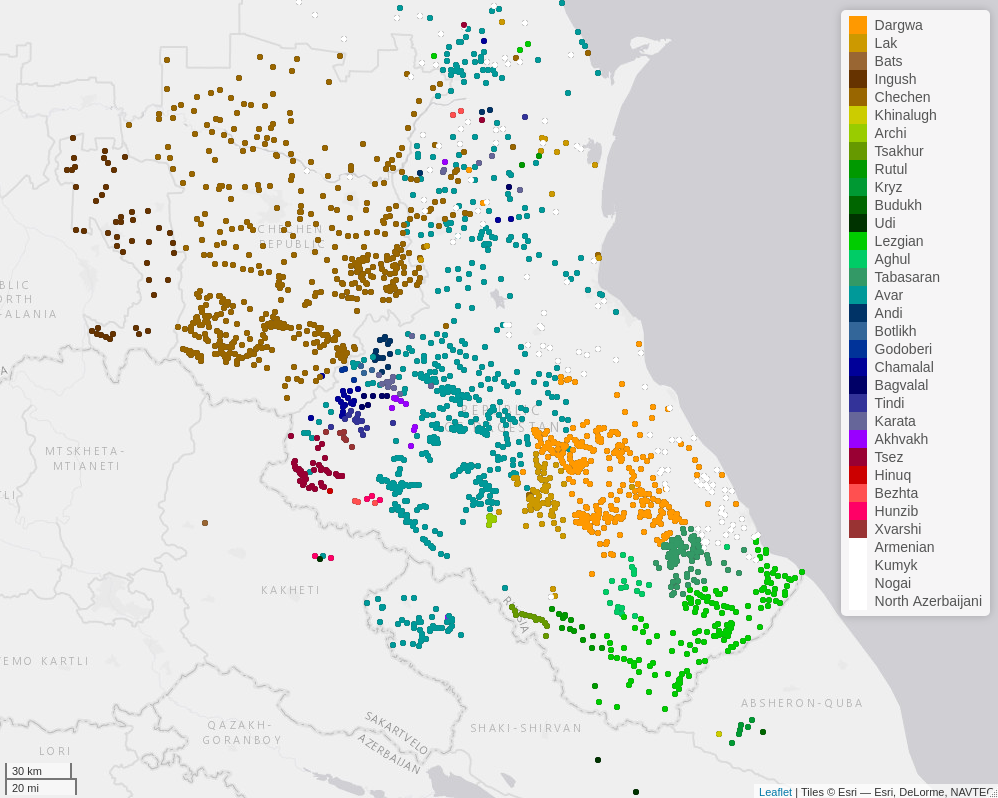
\includegraphics[scale=0.5]{images/all.png}}
\end{figure}

Большинство населенных пунктов, говорящих на языках семьи, находится в одной из четырех кавказских республик: Чечня, Ингушетия, Дагестан и Азербайджан. Некоторые языки и диалекты находятся за пределами России в соседних государствах, например бацбийский язык в Грузии, и хиналугский, закатальский аварский и несколько лезгинских языков на севере Азербайджана. На удинском языке говорят в Грузии и в Азербайджане. В разных странах имеются дагестанские диаспоры, например, в Турции с 19-го века проживает лезгинское сообщество \citep{moor1985}. В Турции и Иордании имеются чеченские и ингушские диаспоры, возникшие в результате депортаций после Кавказской войны \citep[4]{nichols2011}. \color{purple}
\par На территории Восточного Кавказа по соседству с носителями нахско-дагестанских языков живут носители кумыкского, ногайского и азербайджанского языков тюркской семьи, грузинского языка картвельской семьи, осетинского и татского языков индоиранской семьи. В Дагестане до сих пор присутствует армянская диаспора, см. исторические переписи в \citep{multidag}, которые отчасти переселились в период до Кавказской войны (подробнее об этом в \citep{magomedkhanovmusaeva2015}). Во всех трёх республиках представлены и русские, хотя на северо-восточном Кавказе их относительно мало по сравнению с другими национальными республиками, где русские по численности преобладают над коренными народами (как, например, в Республике Коми), и проживают они почти исключительно в городах.\footnote{По данным Всероссийской переписи населения 2010-го года \citep{vpn2010}.}
\par Нахско-дагестанская семья считается одной из трёх коренных языковых семей Кавказа, помимо западно-кавказской (или абхазо-адыгской) и южно-кавказской (или картвельской) семей. Предполагается, что предки нахско-дагестанских народов изначально жили на юге от Главного Кавказского Хребта, а именно в центрально-восточной части Закавказья \citep[317]{schulze2013}, откуда они постепенно распространились по нынешней территории. Высокогорный Дагестан при этом был населен уже в конце раннего неолитического периода (примерно 7500 -- 7000 лет назад);\footnote{В разных местах в Дагестане были найдены и следы первобытного человека ашельского и мустьерского периодов нижнего и среднего палеолита \citep[12--13]{ataevetal1967}.} в раскопках на территории селения Чох (Гунибский район) были найдены остатки зерновых культур, таких как пшеницы и ячменя \citep{amirkhanov1987}. Названия некоторых злаков можно реконструировать для нахско-дагестанского праязыка, датировка которого варьирует от 5000 \citep[21]{koryakov2006} до 6000-8000 лет \citep{nicholsrange}, что подтверждает древность семьи и их проживания на данной территории.
\par В разные периоды на нахско-дагестанские языки влияли разные соседние и внешние языки. Северо-восточный Кавказ входил в состав Персидской империи во время государства Сасанидов, т.е. с \textsc{iii} по \textsc{vii} век \citep[121]{ataevetal1967}. Язык империи был среднеперсидский, и в современных нахско-дагестанских языках отмечены заимствования, которые связывают именно со среднеперсидским периодом, например: \textit{warani} `верблюд' в бежтинском языке \citep{wold15}. После того как сасанидов сменили тюрки-хазары, персидский язык влиял уже как более отдаленный, но все еще важный культурный язык, особенно на юге региона. В лезгинских языках отмечается использование персидских грамматических элементов, например, употребление комплементайзера \textit{ki} в удинском \citep{lander2014}, в хиналугском \citep{daniel2013} и других языках. Впрочем, те же единицы встречаем и в азербайджанском языке, который сильно влиял на языки южного Дагестана и на который персидский в своей очереди оказывал большое влияние, см. базу данных о заимствованной из тюркских языков морфологии в нахско-дагестанских языках \citep{aristova}. Можно предполагать, что персидское влияние было в значительной степени опосредовано азербайджанского языка. 
\par Огузы (предки, в частности, современных турков и азербайджанцев) появились на территории Азербайджана примерно в \textsc{x} веке, во время сельджукской экспансии \citep[162--166]{johanson2006}. Собственно азербайджанский язык сформировался позже, на основе кыпчакских и огузских языков, но <<с преобладанием огузских элементов>> \citep[78]{shiraliev1958}. На юге Дагестана азербайджанский служил языком межэтнического общения, и до сих пор многие носители лезгинских языков владеют, помимо родного и русского языков, также и азербайджанским, см. данные в \citep{multidag}. В других регионах Восточного Кавказа роль лингва франка выполняли аварский, кумыкский и ногайский языки \citep[72--74]{chirikba2008}. 
\par Кыпчаки, предки современных кумыков, появились на Северном Кавказе в \textsc{xi} веке \citep[148]{piotrovksij1988}. Ногайцы (другой кыпчакский народ) появились в регионе намного позже, согласно Л. Йухансон после распада Золотой Орды в \textsc{xiii} веке \citep[162--166]{johanson2006}. На территории Дагестана и современных Чечни и Ингушетии кыпчаки селились в основном на равнине, где играли важную роль в торговых отношениях. Р. Виксман называет пять важных торговых центров и языки, на которых там преимущественно говорили: Моздок (ногайский), Кизляр (ногайский), Буйнакск (кумыкский), Хунзах (аварский) и Дербент (азербайджанский) \citep[58--59]{wixman1980}, см. рисунок \ref{fig:ecmark}. Эти <<рыночные языки>> представляют собой языки, которые носители разных нахско-дагестанских языков в первую очередь усваивали в качестве второго языка, причем не только на базаре, но и во ходе отходничества, сезонных миграций с гор на равнину (см. подробное описание миграционных процессов в Дагестане в \citep[30--39]{karpovkapustina2011}).

\begin{figure}[h]
\centering
\caption{Нахско-дагестанские языки по селам и языки рынков}
\label{fig:ecmark}
\vspace{0.5cm}
\fbox{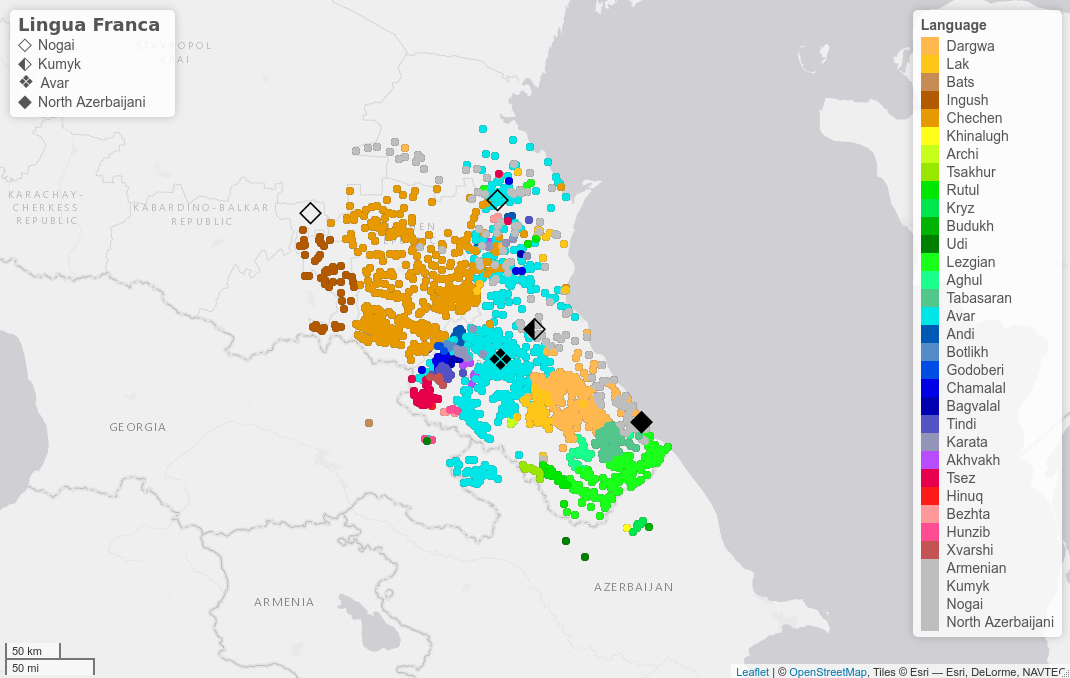
\includegraphics[scale=0.5]{images/ecmark.png}}
\end{figure}

% мне немного кажется что лучше "языки рынков". и еще у меня есть любимая ссылка (которая почему-то не нравится НР) на понятие cardinal market, которое я услышал в одной лекции по истории средневековой англии - мне кажется, она бы очень скрасила это обсуждение - Wrightson, Keith. (2000) Earthly Necessities. Economic Lives in Early Modern Britain. Yale University Press. Очень похоже на наши Кумух, Дербент и проч, мне кажется. Если понравится, то стр 94 (я слушал только устную лекцию, книгу не видел, но это страница, которую мне кажется прислал автор лекции)

Важным внешним языком для Восточного Кавказа является арабский. В конце \textsc{vii} века арабы захватили Дербент и начали миссионерскую деятельность на Северном Кавказе. Арабский халифат просуществовал недолго, но процесс исламизации продолжался и был завершен в \textsc{xv} веке. 
\par В период исламизации появляются первые письменности для нахско-дагестанских языков на основе арабского алфавита. Исламская культура и письменность открыли для нахско-дагестанских народов литературу других мусульманских стран \citep[150]{magomedova2017}. Некоторые мотивы местного фольклора находят параллели в тюркских, иранских и других языках. Сказки часто начинаются с устойчивой формулы <<было, не было>>, которую находим и в персидском, тюркских и балканских языках \citep[355--356]{friedman2000}. 
% у меня ощущение, что эта формула не равно распространена по дагестану. зато кажется есть в грузинском. не уверен, что это такой яркий пример; я бы написасл "В сказках некоторых народов Дагестана..." 
Также широко встречаются анекдоты про Моллу (или Ходжу) Насреддина и другие распространенные на Востоке фольклорные мотивы. В \citep{adzhiev1991intro} отмечается, что влияние арабской исламской культуры на местную литературу и фольклор сильнее всего проявляется на юге Дагестана, с центром вокруг Дербента, а к северо-западу уменьшается. В противоположную сторону идет распространение домусульманских элементов, таких как, например, истории про нартов, которые представлены в том числе у чеченцев \citep[213--215]{jaimoukha2005}, аварцев и кумыков, тогда как на юге они отсутствуют вовсе \citep[19]{adzhiev1991epos}. Влияние собственно арабского языка прослеживается преимущественно в лексике. Большинство терминов, связанных в первую очередь с религией, но также с политикой, философией и наукой имеют арабское происхождение, ср. например \citep{chumakina2009}, \citep{comriekhalilov2009}.
\par Помимо арабского роль престижного внешнего языка выполняет русский язык, хотя он появился на Кавказе относительно недавно. Значительное влияние русского языка начинается только в двадцатые -- тридцатые годов \textsc{xx} века, с создания советских школ и внедрения обязательного школьного образования \citep{dobrushina2019}. Изначально русским владели в основном мужчины, которые служили в армии или работали на государственных или административных должностях (ibid.), но по мере урбанизации и развития школьной системы (четырехлетние школы постепенно заменяли на восьмилетние, потом на десятилетние, становилось более приемлемым отпускать в школу девочек) русский за относительно короткий период стал первым единым лингва франка для всего региона. В Дагестане появился собственный, дагестанский вариант русского языка, некоторые особенные свойства которого обсуждаются в \citep{danieletal2010}. Влияние русского языка на местные языки проявляется в основном в лексике, в терминологических заимствованиях, связанных с распространением современных технологий. Влияние грузинского и армянского языков, крупных соседей со старой литературной традицией, тоже засвидетельствовано, но оно изучено в основном по отношению к тем нескольким языкам, на которые они оказали особенно большое влияние, например цезские, бацбийский и удинский языки. Их влияние на другие нахско-дагестанские языки, по-видимому, ограничено.
\par Нахско-дагестанские языки подвергались влиянию не только внешних, неродственных языков. В Дагестане традиционно было распространено соседское многоязычие, при котором носители владели несколькими (до пяти) местными языками (считая языки тюркских соседей), которые они осваивали в ходе торговли и сезонных работ, связанных, в том числе, со скотоводческими практиками. Про конкретные паттерны традиционного соседского многоязычия в целом в Дагестане мало что известно абсолютно достоверно. Первая попытка к систематическому изучению паттернов многоязычия была предпринята только недавно, см. \textit{Атлас многоязычия в Дагестане} \citep{multidag} и описание проекта в \citep{dobrushina2011}. Данные Атласа в основном описывают ситуацию в рамках временного периода от конца \textsc{xix} века до сегодняшнего дня. Соседское многоязычие при этом практически исчезло: как показывают \citep{dobrushina2019}, знание соседних и местных языков у молодых дагестанцев по сравнению со старшими поколениями очень ограничено. Среди местных языков особое место занимает аварский язык, который служил языком межэтнического общения для носителей цезских, андийских и нескольких других ареально близких языков и который до сих пор преподается в школе в качестве <<родного языка>> носителям бесписьменных языков. В связи с этим статусом аварский язык сильно влиял на эти языки, что отражается в многочисленных заимствованиях (см., например, подробнее о языковых контактах конкретно андийцев с аварским языком в \citep{khalidova2006}). Литературный даргинский язык (который основан на акушинского диалекта) служит такого рода <<родным языком>> для носителей разных даргинских идиомов, которые могут сильно отличаться от акушинского.
\par Выше изложенный обзор, естественно, представляет некоторое упрощение ситуации многоязычия на Восточном Кавказе. Хотя влияние рыночных языков в основном концентрировалось в определенных регионах, границы не абсолютны, и точных данных о том, где говорили на каких языках и каким типом многоязычия они характеризовались (только пассивное, пассивное и активное, свободное владение и т.д.), пока очень мало. При этом русский язык в качестве общего лингва франка с большой скоростью уничтожает следы старых паттернов \citep{dobrushina2019}. Для настоящего исследования важно, что, хотя систематическое исследование конвергенции нахско-дагестанских языков с местными тюркскимим языками остается задачей будущего, данные отдельных работ в целом подтверждают то, что влияние разных тюркских языков отмечено в определенных ареалах и что азербайджанский на юге влиял сильнее чем кумыкский и ногайский на севере и в центральном Дагестане. При этом в кумыкском языке отмечается обратное влияние нахско-дагестанских языков (см., например, \citep{selimova2016} о нахско-дагестанских заимствованиях в кумыкском языке), что также указывает на несколько иной статус кумыкского языка по сравнению с азербайджанским. 
\par Для нас важны именно контакты с тюркскими языками, поскольку эвиденциальность как часть видо-временной системы --- считается древним признаком тюркской грамматики \citep[127]{friedman2018}, тогда как в русском и арабском языках она отсутствует. В грузинском и армянском, влияние которых ограничивается в основном языками, находящимися с ними в непосредственном соседстве, категория вероятно появилась под влиянием тюркских языков и обладает разной степенью грамматикализованности, см. обсуждение в \citep{boeder2000}, \citep{kozintseva2000} и \citep{donabedian2001}. Стоит отметить, что категория эвиденциальности также присутствует в персидском языке. Согласно Й. Сопер, эвиденциальное значение персидского перфекта в целом представляет собой периферийный элемент глагольной парадигмы, который, вероятно, заимствован из азербайджанского или турецкого языка \citep[356--358]{soper1987}. Впрочем, насколько нам известно, вопрос о происхождении именно эвиденциальной функции персидского перфекта не был изучен подробно.

\section{Эвиденциальность в нахско-дагестанских языках} \label{sec:ndevid}

Нахско-дагестанские языки --- языки эргативного строя (субъект переходных глаголов кодируется эргативным падежом, а объект переходных и субъект непереходных глаголов --- абсолютивом, который имеет нулевое маркирование), с преимущественно суффиксальной, агглютинативной морфологией, хотя и в именной, и в глагольной парадигме встречаются элементы флексии. Для языков характерны богатые словоизменительные парадигмы, см. \citep{kibrik2003} об именной морфологии и \citep{forker2018intro} о глагольной. Глагольная парадигма состоит из синтетических и аналитических форм. При этом аналитических форм обычно намного больше, чем синтетических, причем последние и сами часто имеют прозрачное аналитическое происхождение (ibid.). В качестве вспомогательного глагола используются связки, бытийные и другие глаголы. Глаголы согласуются по роду.\footnote{В литературе чаще всего используется слово <<класс>>, см. обсуждение употребления терминов в \citep[155]{vandenberg2005}.} При наличии согласовательного слота глаголы согласуются с абсолютивным аргументом. Чаще всего согласовательный слот является префиксальным, но встречаются и показатели в инфиксальной позиции. Наличие слотов для согласования варьируется. В даргинском большая часть глаголов обладает слотом для классного согласования, ср. \citep{sumbatova2010}, тогда как в андийском языке <<согласуемые глаголы>> составляют скорее меньшинство глагольного лексикона.
\par Во многих языках у глаголов выделяются перфективные, имперфективные и некоторые другие виды основ, которые определяют их возможные сочетания с словоизменительными аффиксами \citep[165--170]{vandenberg2005}. Временные формы часто совмещают временное и видовое значение (например, настоящее прогрессивное или прошедшее завершенное). Другие наклонения кроме изъявительного включают в себя императив, юссив (императив третьего лица --- <<пусть он(а) сделает>>), см. \citep{dobrushina2012}, и гортатив (императив первого лица), прохибитив, и оптатив. Также отмечены эвиденциальность (о которой подробнее ниже), модальность и миративность. Таксисные отношения между клаузами выражауются преимущественно конвербами, которые используются как для подчинения, так и для сочинения клауз \citep{kibrik2007}. Часто встречаются цепочки конвербных клауз в нарративах, так называемое clause chaining, ср. \citep{nedjalkov1995}, \citep{nicholspeterson2010}. При этом распространен синкретизм финитных и нефинитных форм. Формы с нефинитными функциями, такие как причастия, конвербы и масдары (номинализированные глаголы) нередко способны выполнять роль главного предиката, см. \citep{kalininasumbatova2007}, \citep{kazenintestelets2004}, \citep{creissels2009}. Немаркированный порядок слов --- SOV. Порядок этот однако не строгий, и им можно манипулировать для организации информационной структуры \citep{belyaevforker2016}. Другие дискурсивные и некоторые синтаксические функции, включая подчинение, сочинение и, например, вопросительность, выполняют многочисленные частицы и клитики.
\par Эвиденциальность в грамматике нахско-дагестанских языков является относительно новой, периферийной категорией, согласно \citep[ix]{authiermaisak2011}. Во многих случаях, формы находятся еще на пути к грамматикализации, а их источники часто вполне очевидны. Тем не менее, категория так или иначе представлена почти во всех языках семьи, и нахско-дагестанские языки часто упоминаются в типологических обзорах эвиденциальности. Эвиденциальность в основном выражается на главном предикате предложения в форме самого глагола или вспомогательного глагола или клитикой. Различаются следующие способы выражения эвиденциальности (см. также подробный обзор в \citep{forker2018evid}):

\begin{itemize}
    \item Формы глагола наподобие перфекта / косвенная засвидетельствованность
    \item Общие прошедшие / прямая засвидетельствованность
    \item Вспомогательные глаголы / разные значения
    \item Частицы / репортатив, инферентив, косвенная засвидетельствованность
\end{itemize}

Эвиденциальные формы в нахско-дагестанских языках впервые были отмечены относительно рано, еще до появления типологической литературы о категории: они упоминаются уже в работах П.К. Услара в конце 19-го века, см. например обсуждение частицы \textit{ila} и заглазные временные формы глагола в грамматике аварского языка \citep{uslar1889avar}. Заглазные формы прошедшего времени отмечаются и во многих грамматиках и очерках советского периода, например, в грамматиках чамалинского языка \citep{bokarev1949chamalal}, гагатлинского диалекта андийского языка \citep{salimov2010}, и бацбийского языка \citep{desheriev1953}. Термин <<перфект>> в данный период встречается реже; исключениями являются, например, работы \citep{tsertsvadze65}, \citep{kibriketal1972} и некоторых других исследователей. С конца 20-го / начала 21-го веков он становится общепринятым и в дескриптивной литературе. 
\par Подробное изучение семантики этих форм началось лишь 20-30 лет назад, когда авторы грамматик стали уделять больше внимания вопросам семантики и синтаксиса грамматических форм (см. грамматики годоберинского \citep{kibriketal1996}, цахурского \citep{tsakhurgram}, багвалинского \citep{bagvalalgram}, ицаринского даргинского \citep{sumbatovamutalov2003}, ингушского \citep{nichols2011}, гинухского \citep{forker2013} и тантынского даргинского \citep{sumbatovalander2014} языков). Появились отдельные исследования, посвященные перфектным формам и эвиденциальности в следующих языках: андийский \citep{kibrik1985}, цахурский \citep{tatevosovmaisak1999}; \citep{maisaktatevosov2007}, багвалинский \citep{tatevosov2003, tatevosov2007}, багвалинский, арчинский и (кубачинский / ицаринский) даргинский \citep{tatevosov2001}, агульский \citep{maisakmerdanova2002}, лакский \citep{friedman2007}, цезский \citep{comriepolinsky2007}, цезские языки в целом \citep{khalilova2011}, чеченский \citep{molochieva2010}, гинухский \citep{forker2014}, рутульский \citep{verhees2017}, лезгинский \citep{greed2017}, ширинский даргинский с учетом других вариантов даргинского \citep{belyaev2018}, аварский \citep{forker2018evidavar}, ахвахский \citep{creissels2018}, удинский \citep{maisak2018} и лезгинские языки \citep{maisaklezgpf}. Первый обзор категории эвиденциальности в нахско-дагестанских языках вышел в свет в 2018-м году \citep{forker2018evid}.
\par Хотя в большинстве нахско-дагестанских языков категория эвиденциальности в целом считается слабо грамматикализованной и периферийной, она очень заметна: сведения о ней имеются даже в кратких описаниях, и в работах из периода когда сам термин эвиденциальность еще не был принят в типологии. Мы предполагаем, что ранние исследователи обнаружили категорию благодаря мета-комментариям носителей. В \citep[234]{nichols2011} отмечается, что носители ингушского языка отчетливо ощущают и комментируют эвиденциальную семантику глагольных форм. Впрочем, это может варьироваться в зависимости от языка: по данным нашей работы с аварским языком и различными диалектами андийского языка, эвиденциальная семантика осознается разными носителями в разной степени (подробнее об этом в разделе \ref{sec:andinarr}).

\subsection{Перфектоиды} \label{sec:perf}
\color{black}
Формы, похожие на перфект, обнаруживаются во всех современных нахско-дагестанских языках, рассматриваемых нами. Вместе с формально и семантически менее маркированной формой прошедшего времени (например Аорист, Претерит или Простое Прошедшее) они составляют ядро системы прошедшего времени в этих языках. Типологически, перфекты ассоциируются с семантикой текущей релевантности (current relevance) --- действие совершилось в прошлом, но  его последствия в том или ином смысле актуальны на момент речи. Как обсуждалось в разделе \ref{sec:pftyp}, текущая релевантность --- обобщенный ярлык, включающий несколько более частных значений. В описаниях нахско-дагестанских языков (за некоторыми исключениями, перечисленными в разделе \ref{sec:ndevid}) чаще всего встречается только результативная функция, причем результатив в узком смысле и результативный перфект не различаются (см. разделы \ref{sec:res} и \ref{sec:cr}). Это затрудняет типологическую атрибуцию данных форм, поскольку узкий результатив представляет собой более ограниченную конструкцию и более ранний этап в развитии, тогда как результативный перфект представляет следующий этап грамматикализации. Хотя, по нашим данным в нахско-дагестанских языках так или иначе представлены все возможные значения текущей релевантности, остается неизвестным, насколько распространены некоторые из них.
\par Помимо различных значений текущей релевантности отмечено значение косвенной засвидетельствованности --- говорящий не был свидетелем события, о котором он рассказывает. Для цахурского и лакского языков описана более сложная эпистемическая семантика, обозначающая отстранение говорящего от передаваемой информации. Оно напоминает определение медиатива, предложенное Ж. Лазаром (см. обсуждение проблем с терминологией в разделе \ref{sec:pftyp}). Часто, но необязательно, такое употребление совпадает с контекстами, в которых говорящий сам не был свидетелем событий, ср. \citep{friedman2000}, \citep{maisaktatevosov2007}. Подобное значение пока описано только для двух языков, причем сами описания плохо сопоставимы. В настоящей работе мы рассматриваем эти формы как <<эвиденциальные>>, хотя допускаем возможность, что они имеют более сложную семантику. Попытка сопоставительного анализа форм, которые по-разному характеризуются в литературе, представлена в третьей главе диссертации.
\par В настоящем разделе сперва мы сравниваем имеющиеся в литературе сведения о всех перефектоподобных, или <<перфектоидных>>, формах, представленных в нахско-дагестанских языках. \color{purple}В разделе \ref{sec:pftyp} (ст. \pageref{perfectoidpage}) мы определили термин <<перфектоид>> как удобный собирательный термин для <<совокупности нахско-дагестанских глагольных форм, похожих на перфект, но которые необязательно имеют ТР (т.е. текущую релевантность) как главное значение>>. Похожими на перфект мы в первую очередь считаем те формы видо-временной парадигмы, которые имеют функцию результатива, текущей релевантности, или заглазного прошедшего (т.е. значение косвенной засвидетельствованности в прошедшем). На втором этапе мы постарались выявить те формы, которые действительно имеют перфектное или результативное происхождение. 
\par Стоит иметь в виду, что в более старых описаниях некоторых языков глагольные формы классифицируются с помощью современных им ярлыков как <<прошедшее заглазное>> без сопровождения описания их употребления. В грамматике рикванинского диалекта андийского языка, например, отмечено <<прошедшее заглазное>> \citep{sulejmanov1957}, которое по нашим полевым данным имеет и результативную функцию. Для тиндинского перфектоида тоже описано только заглазное значение в \citep{magomedova2012}, тогда как Ж. Отье фиксирует и результативное значение \citep{authiertindi}. Сведения о семантике форм поэтому нужно считать крайне приблизительными --- отсутствие описания определенного значения не значит, что этого значения действительно нет, и для многих языков эта тема требует дальнейшего исследования. С другой стороны, в тех случаях, когда присутствие какого-то значения отмечается, не всегда понятно, на чем это основано, и в какой степени это значение распространено и приемлемо. Несмотря на неполноту данных, в нескольких отдельных случаях можно подтвердить отсутствие или присутствие определенных значений.

\subsubsection{Формальные свойства} \label{sec:pfform}

В общей сложности было рассмотрено 65 формы из 42 разных языковых вариантов, включая все те идиомы, которые традиционно считаются различными языками, а также 13 дополнительных диалектов. Мы нашли 61 <<перфектоидов>> и четыре суффикса неизвестного происхождения (см. ниже), которые выражают подобную семантику. В некоторых языках наличествует две или три формы. Скорее всего наш список неполон для многих рассматриваемых языков. Отметим, что в случае более подробных описаний глагольной парадигмы, как правило, обнаруживается более одной формы. Таблица \ref{tab:pform} суммирует результаты анализа их морфологической структуры. 

\begin{table}[ht]
\caption{Формальная структура нахско-дагестанских перфектоидов}
\label{tab:pform}
\vspace{0.2cm}
\begin{center}
\begin{tabular}{l|llll|l}
          & Копула      & Лицо & Без всп. гл. & Всп. гл. & Итого       \\ \hline
Конверб   & \textbf{26} & 8    & 8            & 1        & \textbf{43} \\
Причастие & 8           & 6    & 1            & 1        & 15          \\
Другое    & 2           & 0    & 4            & 0        & 6           \\ \hline
Итого     & \textbf{36} & 14   & 13           & 2        & 61         
\end{tabular}
\end{center}
\end{table}

Чаще всего формой возглавляет копула, т.е. дефектный вспомогательный глагол со значением <<есть, имеется>> в настоящем времени, который также используется при неглагольной предикации. Конструкция с полноценным вспомогательным глаголом, сохраняющим словоизменительную парадигму, встречается только в одном языке. В даргинских идиомах на месте копулы используются предикативизирующие клитики, выражающие согласование по лицу (см. подробнее в разделе \ref{sec:pfpers}). Во многих случаях где отсутствует вспомогательный элемент, его присутствие на более раннем этапе в диахронии можно предполагать с некоторой уверенностью. Лексический глагол преимущественно появляется в форме конверба, и реже в причастной форме. Отмечено две формы с лексическим глаголом в форме результативной основы, и четыре суффиксов неизвестного происхождения или статуса (т.е. <<другое>>). Ниже мы рассмотрим все варианты и их особенности по отдельности.\footnote{Полная таблица со всеми данными о формах доступна по ссылке \url{https://github.com/sverhees/dissertation_evidentiality}.}

\paragraph{Копула} \label{sec:pfcop}

В 12 языках основной перфектоид сохраняет свою (предполагаемо) исходную аналитическую структуру из конверба и копулы полностью. Эти языки при этом относятся к разным ветвям семьи, см. таблицы \ref{tab:pfcvbcop1} и \ref{tab:pfcvbcop2}. Копула, как правило, дефектная форма, которая выражает настоящее время по умолчанию и не спрягается. При неглагольной предикации, например, в прошедшем времени эти формы заменяются формой бытийного глагола. В бежтинском языке копулу можно (но необязательно) опускать в значении косвенной завсидетельствованности, а в значении текущей релевантности --- нельзя \citep[46]{khalilova2011}. Возможно это является первым шагом к функциональной дифференциации КЗ и ТР, но пока оппозиция несимметричная, мы классифицировали бежтинскую форму как имеющую копулу (впрочем, для цезских языков более характерно опущение копулы, см. раздел \ref{sec:pfzero}).
\par Лексический глагол в целом преимущественно появляется в форме конверба. Обычно это касается форм, которые, помимо перфектоида и других синтетических форм, используются как общий конверб, обозначая первый этап сложного действия или способ действия. Такого рода конвербы встречаются в цепочках клауз для продвижение нарратива (converb chaining) \citep{nedjalkov1995}. В отдельных языках и описаниях эти конвербы называются по-разному, в том числе перфективный конверб и деепричастие прошедшего времени. В составе перфектоидов не встречаются специализированные конвербы, которые передают более узкие таксисные значения, например, <<до того как>>, и т.д.\footnote{Терминология варьируется у разных авторов. Аварский общий/перфективный конверб на \textit{-un} называется в \citep{forker2018evidavar} anterior converb; Крейссель применяет термин anterior к специализированным конвербам маркированного предшествования \citep[127--128]{creissels2012}.}

\begin{table}[ht]
\caption{Полностью аналитические формы с конвербом и копулой (I)}
\label{tab:pfcvbcop1}
\vspace{0.2cm}
\begin{center}
\begin{tabular}{ll|ll}
\multicolumn{2}{l|}{Форма} & Язык      & Источник            \\ \hline
-un  	&	cm-ugo	&	аварский	&	\citep{mallaeva2007}	\\
{[}cvb	&	cop{]}	&	(литературный)	&		\\
-eːhe 	&	gʷeda 	&	ахвахский	&	\citep{magomedbekova1967}	\\
{[}cvb	&	cop{]}	&	(северный)	&		\\
-oː/eː/aː/iː/ereː/areː(-hi/he/ho)	&	godi	&	ахвахский	&	\citep{creissels2018}	\\
\end{tabular}
\end{center}
\end{table}

\begin{table}[H]
\caption{Полностью аналитические формы с конвербом и копулой (II)}
\label{tab:pfcvbcop2}
\vspace{0.2cm}
\begin{center}
\begin{tabular}{ll|ll}
\multicolumn{2}{l|}{Форма} & Язык      & Источник            \\ \hline
{[}cvb 	&	cop{]}	&	(ахахдеринский)	&		\\
-cm-o 	&	ek'ʷa 	&	багвалинский	&	\citep{maisaktatevosov2001}	\\
{[}cvb	&	cop{]}	&	(кванадинский)	&		\\
-na 	&	gey	&	бежтинский	&	\citep{khalilova2011}	\\
{[}cvb	&	cop{]}	&	(бежтинский)	&		\\
-ida // -a/-u 	&	ida 	&	ботлихский	&	\citep{alexeyevverhees2019}	\\
{[}pf{]} // {[}cvb	&	cop{]}	&	(ботлихский)	&		\\
-dːu 	&	ide	&	чамалинский	&	\citep{bokarev1949chamalal}	\\
{[}cvb	&	cop{]}	&	(гадыринский)	&		\\
-un 	&	lo/li 	&	гунзибский	&	\citep{vandenberg1995}	\\
{[}cvb 	&	cop{]}	&	(гунзибский)	&		\\
-cm-oxa 	&	ida	&	каратинский	&	\citep{magomedbekova1971}	\\
{[}cvb 	&	cop{]}	&	(каратинский)	&		\\
-un 	&	goli 	&	хваршинский	&	\citep{khalilova2009}	\\
{[}cvb 	&	cop{]}	&	(инхокваринский)	&		\\
-unu 	&	cm-ur 	&	лакский	&	\citep{friedman2007}	\\
{[}cvb 	&	cop{]}	&	(литературный)	&		\\
pf.stem 	&	a // ʔa	&	рутульский	&	\citep{maisaklezgpf}	\\
{[}cvb 	&	cop{]}	&	(литературный)	&		\\
pf.stem 	&	wo-cm	&	цахурский	&	\citep{maisaktatevosov2007}	\\
{[}cvb 	&	cop{]}	&	(мишлешский)	&		\\
pf.stem 	&	wo-cm-un	&	цахурский	&	\citep{maisaktatevosov2007}	\\
{[}cvb 	&	cop{]}	&	(мишлешский)	&		\\
\end{tabular}
\end{center}
\end{table}

В двух языках такая конструкция образует узкую результативную конструкцию, противопоставленную более грамматикализованному перфектоиду с опущенной копулой. Редуцированная форма в этих случаях вероятно восходит к аналитической структуре, см. \citep{tatevosov2001} для обсуждения арчинского случая, и раздел \ref{sec:parad} ниже о чеченской парадигме по сравнению с другими языками нахской группы. Здесь мы называем такие формы <<вторичными>> (см. таблицу \ref{tab:pfcvbcopsec}), поскольку они более ограничены в своем употреблении и занимают менее центральное место в парадигме чем перфектоиды с функциями текущей релевантности или косвенной засвидетельствованности, с которыми они сосуществуют. Слово вторичный тем самым не имеет отношения к диахроническим связям: узкие результативы наоборот предшествуют остальным перфектоидным формам.

\begin{table}[ht]
\caption{Вторичные полностью аналитические формы с конвербом и копулой}
\label{tab:pfcvbcopsec}
\vspace{0.2cm}
\begin{center}
\begin{tabular}{ll|ll}
\multicolumn{2}{l|}{Форма} & Язык      & Источник        \\ \hline
-li 	&	cm-i 	&	арчинский	&	\citep{tatevosov2001}	\\
{[}cvb	&	cop{]}	&		&		\\
-na 	&	cm-u 	&	чеченский	&	\citep{molochieva2010}	\\
{[}cvb	&	cop{]}	&	(литературный)	&		\\
\end{tabular}
\end{center}
\end{table}

В 8 языках копула в конструкции с конвербом подверглась морфологизацией, и стала суффиксом прозрачной этимологии (ср. формы в таблице \ref{tab:pfcvbcopred}). Это касается в основном лезгинских языков, нескольких андийских языков, и ингушского языка. Интересный случай представлен в крызском языке: перфектоид с суффиксом \textit{–ǯija} (который членится на суффикс конверба (\textit{ǯi}) и копулы (\textit{ja}) выражает результатив в узком понимании, а его редуцированный вариант \textit{ǯa} выражает текущую релевантность \citep[19]{maisaklezgpf}. 

\begin{table}[ht]
\caption{Формы на основе конверба с морфологизированной копулой}
\label{tab:pfcvbcopred}
\vspace{0.2cm}
\begin{center}
\begin{tabular}{ll|ll}
\multicolumn{2}{l|}{Форма} & Язык      & Источник               \\ \hline
-naa/naja	&		&	агульский	&	\citep{maisaklezgpf}	\\
{[}cvb.cop{]}	&		&	(хпюкский)	&		\\
-eːda / -iːda 	&		&	чамалинский	&	\citep{bokarev1949chamalal}	\\
{[}cvb.cop{]}	&		&	(гакваринский)	&		\\
-dːa	&		&	чамалинский	&	\citep{bokarev1949chamalal}	\\
{[}cvb.cop{]}	&		&	(гигатльский)	&		\\
-á/ú-da 	&		&	годоберинский	&	\citep{dobrushinatatevosov1996}	\\
{[}cvb-cop{]}	&		&	(годоберинский)	&		\\
-na<cm>(y) 	&		&	ингушский	&	\citep{nichols2011}	\\
{[}cvb.cop{]}	&		&	(литературный)	&		\\
dža	&		&	крызский	&	\citep{authier2009}	\\
{[}cvb.cop{]}	&		&	(алыкский)	&		\\
džija-cm	&		&	крызский	&	\citep{authier2009}	\\
{[}cvb.cop{]}	&		&	(алыкский)	&		\\
-nwa	&		&	лезгинский	&	\citep{haspelmath1993}	\\
{[}cvb.cop{]}	&		&	(литературный)	&		\\
-na	&		&	табасаранский	&	\citep{maisaklezgpf}	\\
{[}cvb.cop{]}	&		&	(литературный)	&		\\
-(w)oː	&		&	тиндинский	&	\citep{magomedova2012};	\\
{[}cvb.cop{]}	&		&	(тиндинский)	& \citep{authiertindi}	\\
\end{tabular}
\end{center}
\end{table}

\par В целом ожидалось бы, что редуцированные формы --- более грамматикализованные, что в принципе подтверждается нашими данными: те формы, которые выражают только узкий результатив (их всего 7) --- менее редуцированные чем те, которые выражают ТР (текущую релевантность) или КЗ (косвенная засвидетельствованность). В 5 случаях они сохраняют аналитическую структуру, а в двух случаях копула морфологизированная, например в крызском языке, где, как обсуждалось выше, узкий результатив относительно менее редуцирован чем основной Перфект. Единственным исключением является годоберинский язык, о котором подробнее в разделе \ref{sec:pfaux}. Стоит здесь отметить, что многие грамматикализованные формы тоже сохраняют аналитическую структуру, т.е., если формы выражает только узкий результатив, высока вероятность, что она нередуцированная, или относительно менее редуцированная, но если форма нередуцированная, это ничего не говорит о ее функции. К тому же, есть редуцированные синтетические формы которые сохраняют узко-результативную функцию помимо остальных. В ботлихском языке редуцированная форма ялвяется вариантом аналитической конструкции: в одном и том же контексте носители могут употреблять полную форму, или использовать копулу как суффикс, который присоединяется прямо к основе, ср. \textit{b-uk'a ida} `был' // \textit{b-uk'-ida}.\footnote{В связи с тем, что полная форма до сих пор представлена в ботлихском языке, и она по всей видимости не отличается от редуцированной формы в функциональном плане, ботлихский Перфект анализируется нами как аналитический.} Впрочем процесс морфологизация, как представлена в ботлихском языке, достаточно уникальная --- в других языках происходит стяжение показателя конверба с копулой, например в лезгинских языках, представленных в таблице \ref{tab:pfcvbcopred}, но также в чамалинском и тиндинском языках андийской группы, а в близкородственном годоберинском языке опускается начальное гласное копулы вместо конвербного суффикса: \textit{-á/ú-da}, от \textit{-á/ú} + \textit{ida}.
\par Причастные перфектоиды встречаются значительно реже чем конвербные (см. таблицу \ref{tab:pform}), и при этом обычно существуют наряду с перфектоидами с конвербом. Единственным исключением является будухский язык лезгинской ветви, в котором отмечен только один, причастный перфектоид. Причастные перфектоиды представлены в языках разных ветвей и разных регионов, и их причастная основа не коррелирует с определенной перфектоидной функцией. Ниже в таблице \ref{tab:ptcpcop} представлены аналитические формы, а в таблице \ref{tab:ptcpredcop} --- формы на причастной основе с редуцированной копулой.

\begin{table}[ht]
\caption{Формы на основе причастия и копулы}
\label{tab:ptcpcop}
\vspace{0.2cm}
\begin{center}
\begin{tabular}{ll|ll}
\multicolumn{2}{l|}{Форма} & Язык      & Источник               \\ \hline
-u-cm 	&	ek'ʷa 	&	багвалинский	&	\citep{maisaktatevosov2001}	\\
{[}ptcp	&	cop{]}	&	(кванадинский)	&		\\
-no-cm-a 	&		&	бацбийский	&	\citep{holiskygagua1994}	\\
{[}ptcp/cvb.cop{]}	&		&		&		\\
-s/š/iš 	&	goɬ 	&	гинухский	&	\citep{forker2013}	\\
{[}ptcp	&	cop{]}	&	(гинухский)	&		\\
-d  	&	i 	&	рутульский	&	\citep{maisaklezgpf}	\\
{[}ptcp 	&	cop{]}	&	(литературный)	&		\\
\end{tabular}
\end{center}
\end{table}

Бацбийский язык включен немного условно в таблицу \ref{tab:ptcpcop}. В описании \citep{holiskygagua1994} форма на \textit{-no} описана как причастие, но в бацбийских текстах данная форма по всей видимости используется как общий конверб (см., например, проанализированные фрагменты в \citep{nichols1981}). При этом мы знаем что явно когнатные формы из других нахских языков (с суффиксом \textit{-na}) выполняют функцию причастия и конверба, а Перфекты анализируются как основаны именно на форме в конвербной функции (ср. \citep{molochievanichols2018}). 

\begin{table}[ht]
\caption{Причастие и редуцированная копула}
\label{tab:ptcpredcop}
\vspace{0.2cm}
\begin{center}
\begin{tabular}{ll|ll}
\multicolumn{2}{l|}{Форма} & Язык      & Источник   \\ \hline
-f-e	&		&	агульский	&	\citep{maisaklezgpf}	\\
{[}ptcp-cop{]}	&		&	(хпюкский)	&		\\
-najef-e	&		&	агульский	&	\citep{maisakmerdanova2016}	\\
{[}ptcp-cop{]}	&		&	(хпюкский)	&		\\
-vi 	&		&	будухский	&	\citep{maisaklezgpf}	\\
{[}ptcp.cop{]}	&		&	(будухский)	&		\\
-bú-da 	&		&	годоберинский	&		\\
{[}ptcp-cop{]}	&		&	(годоберинский)	&		\\
\end{tabular}
\end{center}
\end{table}

Основой для перфектоида в хиналугском языке служит результативная основа лексического глагола. Результативная основа при этом не совпадает ни с какой другой формой, например, с конвербом / прошедшим, как в цахурском и тиндинском языках. Копулы, которые образуют перфектоиды в хиналугском, в неглагольной предикации используются именно в поссессивных конструкциях, согласно \citep[162--164]{kibriketal1972}. 

\begin{table}[H]
\caption{Основа и копула}
\label{tab:stemcop}
\vspace{0.2cm}
\begin{center}
\begin{tabular}{ll|ll}
\multicolumn{2}{l|}{Форма} & Язык      & Источник   \\ \hline
res.stem-(q)omæ	&		&	хиналугский	&	\citep{kibriketal1972}	\\
{[}stem-cop{]}	&		&		&		\\
res.stem-athmæ	&		&	хиналугский	&	\citep{kibriketal1972}	\\
{[}stem-cop{]}	&		&		&		\\
\end{tabular}
\end{center}
\end{table}

Форма  \textit{(q)omæ} дополнительно выражает пространственный дейксис, указывающая на то, что референт находится ниже говорящего, тогда как \textit{athmæ} --- нейтральна в этом плане. Отмечено в \citep[178]{kibriketal1972}, что перфектоид со связкой \textit{(q)omæ} <<иногда имеет оттенок заглазности>>. Такая формулировка подразумевает что в данном случае эвиденциальная функция всего лишь слабая импликатура, в связи с тем эта форма была классифицирована как не имеющая эвиденциальную функцию.

\paragraph{Личные клитики} \label{sec:pfpers}

В даргинских идиомах вместо копул встречаются личные клитики. Личные клитики похожи на копулы в других нахско-дагестанских языках в таком плане, что они образуют предикаты: они употребляются при неглагольной предикации и в случае перфектоидов образуют финитные формы от конвербов (таблица \ref{tab:cvbpers}) или причастий (таблица \ref{tab:ptcppers}). Тем не менее, нельзя их приравнять к копулам в других языках, поскольку личные клитики могут сочетаться с копулами. К тому же, остается недоказанным, что личные клитики исходно являются глаголами:

\begin{displayquote}
<<Можно предположить, что на более ранней стадии развития языка клитики действительно функционировали как самостоятельные словоформы и занимали при этом позицию предиката. Однако предположение о глагольном происхождении личных клитик, сколь бы разумным оно ни казалось, пока остается необоснованным, так как до сих пор ни для лакской, ни для даргинской группы не выдвинуто конкретных предположений о том, что за глаголы могли быть источниками личных клитик и что с ними происходило.>>\\
\citep[586]{sumbatovalander2014}.
\end{displayquote}

Личные клитики в даргинских идиомах, в отличие от копул в других языках, в составе перфектоида не редуцируется. Только в одном идиоме (а именно в ширинском) засвидетельстовано опущение клитики в третьем лице, но в отличие, например, от болгарского языка, опущение формы третьего лица не маркирует функциональную разницу между двумя перфектоидами (о специфике болгарской системы, см. ССЫЛКА) --- в ширинском даргинском наличествует три перфектоида, а клитика третьего лица опускается только в специализированной форме текущей релевантности на основе короткой формы причастия, тогда как остальные формы образуются от других нефинитных форм.\footnote{О.И. Беляев считает в том числе опущение клитики в третьем лице поводом отнести ширинский Перфект к синтетическим формам \citep[95]{belyaev2018}, но для наших сопоставительных целей на уровне всей семьи, мы решили его все-таки включить в аналитические формы, поскольку он кроме в контексте третьего лица явно состоит из полной нефинитной формы и нередуцированной формы клитики, в отличие от остальных синтетических форм в нашей выборке, у которых ни одной утвердительной формы не сохраняет исходную, композициональную структуру.}

\begin{table}[ht]
\caption{Конверб и личная клитика}
\label{tab:cvbpers}
\vspace{0.2cm}
\begin{center}
\begin{tabular}{ll|ll}
\multicolumn{2}{l|}{Форма} & Язык      & Источник   \\ \hline
-ib-li={[}person{]}  	&		&	даргинский	&	\citep{belyaev2018}	\\
{[}cvb=person{]}	&		&	(акушинский)	&		\\
-ib-li={[}person{]}	&		&	даргинский	&	\citep{belyaev2018}	\\
{[}cvb=person{]}	&		&	(аштынский)	&		\\
-li=ra/ri/sa<cm>i 	&		&	даргинский	&	\citep{mutalov2018}	\\
{[}cvb=person{]}	&		&	(литературный)	&		\\
-ib-li={[}person{]} 	&		&	даргинский	&	\citep{belyaev2018}	\\
{[}cvb=person{]}	&		&	(ицаринский)	&		\\
-ib-li={[}person{]} 	&		&	даргинский	&	\citep{belyaev2018}	\\
{[}cvb=person{]}	&		&	(кайтагский)	&		\\
-ib-li={[}person{]} 	&		&	даргинский	&	\citep{belyaev2018}	\\
{[}cvb=person{]}	&		&	(кубачинский)	&		\\
-ib-li=da/di/ca<cm>i 	&		&	даргинский	&	\citep{belyaev2018}	\\
{[}cvb=person{]}	&		&	(ширинский)	&		\\
-ib-li={[}person{]} 	&		&	даргинский	&	\citep{belyaev2018}	\\
{[}cvb=person{]}	&		&	(тантынский)	&		\\
\end{tabular}
\end{center}
\end{table}

В разделе \ref{sec:pfcop} мы отметили, что в принципе нет корреляции между формой лексического глагола (причастие или конверб) и функцией, которую выполняет перфектоид. В даргинском дело обстоит немного иначе: результативную функцию исключительно выполняют конвербные формы, при чем причастные формы преимущественно специализированы на какую-то одну функцию: ТР, экспериентив (частное значение из семейства ТР), или КЗ, тогда как конвербные формы в целом сочетают разные функции. О.И. Беляев в связи с этим предполагает, что можно реконструировать результативную конструкцию из конверба и личной клитики для прото-даргинского уровня \citep[107, 113]{belyaev2018}, и дальше эта конструкция развивалась по-своему в разных идиомах. Помимо этого, Беляев реконструирует Перфект на причастной основе, который только в ширинском остался Перфектом (т.е. специализированная форма ТР), а в других идиомах перешел в Аорист или исчез. 

\begin{table}[ht]
\caption{Причастие и личное окончание}
\label{tab:ptcppers}
\vspace{0.2cm}
\begin{center}
\begin{tabular}{ll|ll}
\multicolumn{2}{l|}{Форма} & Язык      & Источник   \\ \hline
-si=ra/ri/sa<cm>i 	&		&	даргинский	&	\citep{mutalov2018}	\\
{[}ptcp=person{]}	&		&	(литературный)	&		\\
-ib={[}person{]} 	&		&	даргинский	&	\citep{belyaev2018}	\\
{[}ptcp=person{]}	&		&	(ицаринский)	&		\\
-ib={[}person{]} 	&		&	даргинский	&	\citep{belyaev2018}	\\
{[}ptcp=person{]}	&		&	(кайтагский)	&		\\
-ib={[}person{]} 	&		&	даргинский	&	\citep{belyaev2018}	\\
{[}ptcp=person{]}	&		&	(кубачинский)	&		\\
-ib-zi-cm=da/di/ca<cm>i 	&		&	даргинский	&	\citep{belyaev2018}	\\
{[}ptcp=person{]}	&		&	(ширинский)	&		\\
-ib=da/di/Ø 	&		&	даргинский	&	\citep{belyaev2018}	\\
{[}ptcp=person{]}	&		&	(ширинский)	&		\\
\end{tabular}
\end{center}
\end{table}

\paragraph{Без вспомогательного глагола} \label{sec:pfzero}

Другой диахронический путь к суффиксальному перфектоиду кроме морфологизации копулы походит через ее опущение. Если копула отсутствует, а перфектоид совпадает с какой-либо из нефинитных форм, не всегда очевидно, что это именно результат опущения. Синкретизм финитных и нефинитных форм может и возникать, когда подчиненная клауза переосмысляется как главная, так что нефинитная форма, которая ее возглавляет, переосмысляется как сказуемое, т.е. <<инсубординация>> (см. типологический обзор этого феномена в \citep{evans2007}). Например, в чеченском языке имеется Перфект с суффиксом \textit{-na}, который тождествен суффиксу Перфективного Конверба. На базе того же конверба и копулы \textit{\textsc{cm}-u} образуется также узкий Результатив. В близкородственном ингушском языке форма, которая состоит из конверба на \textit{-na} и когнатной копулы \textit{\textsc{cm}-y}, передает значения текущей релевантности, результатива и косвенной засвидетельствованности. В связи с этим нам кажется вероятным, что чеченский Перфект восходит к той структуре, которая сохраняется в ингушском, а копула была утрачена в процессе грамматикализации значения текущей релевантности. В гинухском и цезском языках перфектоиды совпадают с конвербом в утвердительных предложениях, однако при отрицании копула снова появляется, так что в этом смысле для утвердительной формы в этих языках можно постулировать копулу.

\begin{table}[ht]
\caption{Нефинитные формы}
\label{tab:nonfin}
\vspace{0.2cm}
\begin{center}
\begin{tabular}{ll|ll}
\multicolumn{2}{l|}{Форма} & Язык      & Источник   \\ \hline
-dːu	&		&	андийский	&	\citep{kibrik1985}	\\
{[}cvb{]}	&		&	(андийский)	&		\\
-d	&		&	андийский	&	\citep{verhees2018}	\\
{[}cvb{]}	&		&	(рикванинский)	&		\\
-j/nij	&		&	андийский	&	(Fieldwork)	\\
{[}cvb{]}	&		&	(зиловский)	&		\\
-li	&		&	арчинский	&	\citep{tatevosov2001}	\\
{[}cvb{]}	&		&		&		\\
-na	&		&	чеченский	&	\citep{molochieva2010}	\\
{[}cvb{]}	&		&	(литературный)	&		\\
-no/n	&		&	гинухский	&	\citep{forker2013}	\\
{[}cvb{]}	&		&	(гинухский)	&		\\
-un	&		&	хваршинский	&	\citep{khalilova2011}	\\
{[}cvb{]}	&		&	(инхокваринский)	&		\\
-no/n	&		&	цезский	&	\citep{khalilova2011}	\\
{[}cvb{]}	&		&		&		\\
<person>-ijo	&		&	удинский	&	\citep{maisak2016}	\\
{[}ptcp{]}	&		&	(ниджский)	&		\\
\end{tabular}
\end{center}
\end{table}

Для андийского языка не удалось выяснить, использовалась ли когда-нибудь в составе перфектоида связка. Если сравнить перфектоиды разных андийских диалектов с перфектоидами других языков андийской группы, кажется очень вероятным, что и в андийском языке когда-то имел место перфектоид, состоящий из конверба и копулы. Тем не менее, несколько факторов мешают нам реконструировать аналитическую структуру с копулой. В андийском языке имется суффиксальный перфектоид на \textit{-dːu}, который совпадает с Общим Конвербом.\footnote{Форма \textit{-dːu} встречается в андийском и гагатлинском диалектах, варианты \textit{-d} (рикванинский) и \textit{-j} (зиловский) на наш взгляд явно представляют собой редукцию формы на \textit{-dːu}. В нижне-андийских диалектах при этом, находим формы иного происхождения.} 
\par Отрицание конверба оформляется сложным суффиксом \textit{-č’igu}, который исторически состоит из отрицательного и конвербного суффиксов: *\textit{-č’i-gu} [\textsc{-neg-cvb}], ср. обсуждение в \citep[202--203]{verhees2019}). При финитном употреблении перфектоида на \textit{-dːu} имеется два разных способа выражения отрицания: тот же суффикс \textit{-č’igu}, и присоединение регулярного отрицания (\textit{-sːu}) к утвердительному суффиксу (\textit{-dːu-sːu}). Конверб же, по всей видимости, отрицается только суффиксом \textit{-č’igu}. Нам кажется вероятным, что суффикс \textit{-dːu} исторически является суффиксом финитной формы, поскольку позиция отрицания после словообразовательного суффикса в целом характерна в андийском языке для финитных форм в отличие от нефинитных (ср. позицию отрицательного элемента в составе \textit{-č’i-gu}). Показатель \textit{-dːu} в свою очередь может восходить к аналитической форме. В чамалинском диалекте с. Гигатль Перфект образуется похожим суффиксом \textit{-dːa}, который появляется в результате стяжения конвербного суффикса \textit{-t’u} и копулы \textit{ida} \citep[105]{bokarev1949chamalal}.

\begin{table}[ht]
\caption{Суффиксы неизвестного происхождения}
\label{tab:suff}
\vspace{0.2cm}
\begin{center}
\begin{tabular}{ll|ll}
\multicolumn{2}{l|}{Форма} & Язык      & Источник   \\ \hline
-wudi	&		&	ахвахский	&	\citep{creissels2018}	\\
{[}pfv.wudi{]}	&		&	(ахахдеринский)	&		\\
-la-{[}person/class{]}	&		&	аварский	&	\citep{saidova2007}	\\
{[}pst.unwit{]}	&		&	(закатальский)	&		\\
-no 	&		&	бацбийский	&	\citep{holiskygagua1994}	\\
{[}ptcp/cvb{]}	&		&		&		\\
-e={[}person{]}	&		&	удинский	&	\citep{maisak2018}	\\
{[}pf{]}	&		&	(ниджский)	&		\\
\end{tabular}
\end{center}
\end{table}

\par Тем не менее, для андийского языка мы не можем восстановить точный путь развития суффикса. Копула в андийском языке (когнат чамалинской \textit{ida}, согласно \citep[57]{gudava1959}) имеет форму \textit{dži / ži / i}, в зависимости от диалекта. Развитие из, например, конвербного суффкиса \textit{-gu} и копулы \textit{dži} в суффикс \textit{-dːu}, с редкой для нахско-дагестанских языков фонемой \textit{/dː/} гораздо менее очевидно чем переход \textit{-t’u} + \textit{ida} в \textit{-dːa}.\footnote{Андийская копула в принципе не употребляется в аналитических формах, кроме как в кванхидатлинском Перфекте, который состоит из Аориста и копулы \textit{dži}.} При этом, если мы принимаем по крайней мере, что \textit{-dːu} является исходно суффиксом финитной формы, остается непонятным, каким путём он перешел в конвербный показатель. Во всех других языках наблюдается только обратный случай, при котором конвербная форма приобретает финитное употребление, например, через опущение копулы. В связи с этим андийские перфектоиды были классифицированы нами как не имеющие в своем составе вспомогательный глагол.
\par Единственная перфектоидная форма в наших данных, которая имеет значение текущей релевантности, но образуется суффиксом неизвестного происхождения, обнаруживается в удинском языке, хотя анализ отрицательных форм позволяет предполагать что происхождение скорее всего аналитическое, ср. \citep[158--160]{maisak2018}. Отметим, что аналогичная форма в кавказских албанских палимпсестов \textsc{v-vi} века не отмечена, в отличие, например, от удинского аориста, аналог которого был представлен уже в старых памятниках кавказской албанской письменности (ibid.). В закатальском диалекте аварского языка имеется суффикс Заглазного Прошедшего \textit{-la}, для которого происхождение также не установлено. Неизвестно, имеет ли эта форма лишь эвиденциальное значение, или у нее есть и другие функции \citep[143--144]{saidova2007}. В ахвахском диалекте села Ахахдере (Азербайджан) помимо обычного Перфекта текущей релевантности имеется эвиденциальный суффикс \textit{-wudi} \citep{creissels2018}. В грамматике \citep{magomedbekova1967}, написанной на материале дагестанских диалектов ахвахского языка, суффикс \textit{-wudi} не упоминается.
\par Как уже было отмечено в разделе \ref{sec:pfcop}, в бацбийском языке есть причастие с суффиксом \textit{-no}, которое также используется как конверб, аналогично когнатам в других нахских языках. Форма при этом совпадает с <<репортативным аористом>>, который состоит из Аориста и суффикса \textit{-no}. Остается не совсем понятным, в результате какого процесса форма на \textit{-no} стала именно Репортативным Аористом (т.е. прошедшее заглазное). Отмечено в \citep{holiskygagua1994} также отмечено, что перфектоидная форма из причастия/конвербы на \textit{-no} и копулы \textit{-\textsc{cm}-a}, упомянутая нами выше в разделе \ref{sec:pfcop}, появляется только в отрицательных контекстах. Стоит отметить, что, в отличие от других нахско-дагестанских языков, отрицание в бацбийском не выражается морфологически на глаголе, а оформляется отрицательной частицей в клаузе. Поэтому форма имеет структуру утвердительной, несмотря на то, что она ограничена отрицательными контекстами. Согласно \citep{holiskygagua1994}, по семантике форма похожа именно на Репортативный Аорист. Нам кажется вероятным, что Репортативный Аорист на \textit{-no} восходит к перфектойдной форме, которая опускала копулу в утвердительном в процессе грамматикализации, но сохранила ее в отрицательном контексте, аналогично ситуации, например, в цезских языках. В пользу такой теории говорит наличие примеров где перфектоидная форма используется с заглазным значением (при чем в утвердительном контексте), ср. пример (\ref{ex:batsperf}).\footnote{Пример из текстов, записанных Ю.Д. Дешериевым \citep{desheriev1953}, глоссы были добавлены Йессе Вихерс Схрёр.}
%проверить как транслитерировать имя

%спросить про сокр.
\lb{ex:batsperf}{\gll giurg	psṭuna-v j-ɦivɁ	joḥ	\textbf{j-i-en-j-a}.\\
Giorgi	woman-{\Erg} {\F}.{\Sg}-four girl {\F}.{\Sg}-give\_birth-{\Pst}.{\Ptcp}-{\F}.{\Sg}-be.lv\\ 
\trans `\textit{Оказывается, что} жена Гиоргия \textbf{родила} четыре девочки.'\\
\footnotesize{\citep{desheriev1953} \hfill бацбийский язык}}

\paragraph{Вспомогательный глагол} \label{sec:pfaux}

Только в одном языке встречаются формы с полноценным вспомогательным глаголом, т.е., спрягаемый бытийный глагол вместо копулы. В годоберинском языке имеется Перфект с эвиденциальным значением, и результативная конструкция. Первая форма образуется от конверба и копулы, вторая от причастия и той же копулы. Обе формы имеют аналог с глаголом `быть' в форме прогрессива вместо копулы.\footnote{Настоящее прогрессивное в годоберинском языке образуется аналитически от прогрессивного конверба и копулы.} Функциональная дистрибуция конвербных форм, судя по описанию в \citep{dobrushinatatevosov1996}, заключается в том, что форма с копулой указывает на незасвидетельствованные события, тогда как форма с глаголом `быть' в форме прогрессива, указывает именно на засвидетельствованные события. Оба при этом сохраняют семантику ТР. Хотя очень часто встречаются формы, которые выражают семантику ТР с оттенком инферентива, и разграничение этих двух функций не всегда можно провести с уверенностью, нам не известны языки, в которых противопоставление по засвидетельствованности выражается именно двумя перфектоидами, вместо перфектоидом с одной стороны, и общее прошедшее с другой. Единственный пример на второй перфектоид который приводится в \citep{dobrushinatatevosov1996}, представлен в примере (\ref{ex:pfpf}).

\lb{ex:pfpf}{\gll den hincːu χʷab-u b-uk'-at-a-da\\
I.{\Erg} door open.{\Pst}-{\Cvb} {\N}-be-{\Prs}-{\Cvb}-{\Cop}\\
\trans `Я открыл дверь.'\\
\footnotesize{\citep[96]{dobrushinatatevosov1996} \hfill годоберинский язык}}

Другой перфектоид, наоборот, не сочетается с действующим субъектом первого лица, ср. \citep[94]{dobrushinatatevosov1996}. Возможно второй перфектоид --- специализированная форма ТР для первого лица, которая используется в избежании известного эффекта первого лица.\footnote{Известно, что формы косвенной засвидетельствованность плохо сочетаются с действующим субъектом первого лица, поскольку человек обычно является свидетелем собственных действий. В связи с этим, наблюдаются разные эффекты первого лица, в плане частотности употребления показателей косвенной засвидетелсьтвованности с субъектом первого лица, но и в плане интерпретации таких конструкций \citep{curnow2002}. Если показатель косвенной завсидетельствованности сочетается с субъектом первого лица, часто возникает интерпретация, что говорящий совершил действие неосознанно, например, потому что он спал или был пьян.} В случае результативной конструкции, наоборот, именно форма со вспомогательным глаголом выражает косвенную засвидетельствованность. Это немного неожиданное парадигматическое отношение, которое требует дальнейшего изучения.

\begin{table}[ht]
\caption{Перфектоид со вспомогательным глаголом}
\label{tab:aux}
\vspace{0.2cm}
\begin{center}
\begin{tabular}{ll|ll}
\multicolumn{2}{l|}{Форма} & Язык      & Источник   \\ \hline
-á/ú 	&	cmV=k'-at-á-da	&	годоберинский	&	\citep{dobrushinatatevosov1996}	\\
{[}cvb 	&	{[}aux-pres-cvb{]}	&	(годоберинский)	&		\\
-bú 	&	cmV=k'-at-á-da	&	годоберинский	&	\citep{dobrushinatatevosov1996}	\\
{[}ptcp 	&	{[}aux-pres-cvb{]}	&	(годоберинский)	&		\\
\end{tabular}
\end{center}
\end{table}


\subsubsection{Семантика} \label{sec:pfsem}

Семантика перфектоидов состоит, с одной стороны, из значений, которые вытекают из составляющих конструкций, таких как лексической семантики или акционального класса глагола, видо-временного значения используемых форм (например копула настоящего времени в сочетании с перфективным конвербом) и управления предиката. Это касается следующих значений (подробнее об отдельных функций см. соответствующие разделы ниже):

\begin{itemize}
    \item результатив (\ref{sec:res})
    \item результативный перфект (\ref{sec:cr})
    \item континуатив (\ref{sec:cr})
\end{itemize}

Помимо этого есть группа значений, возникающих из импликатур (процесс развития импликатурных значений обсуждалось в разделе \ref{sec:pftyp}. Основные из них следующие:

\begin{itemize}
    \item недавнее прошедшее (\ref{sec:cr})
    \item эвиденциальность (\ref{sec:semevid})
    \item эпистемическая модальность (\ref{sec:semevid})
\end{itemize}

\textbf{Миративное} значение, описанное для перфектоидов эвиденциального типа в разных языках, может в свою очередь восходить к недавнему прошедшему или эвиденциальности (конкретно к инферентиву), как было отмечено в разделе \ref{sec:pftyp}. Значение \textbf{экспериентива} (\ref{sec:cr}), который вместе с результативным перфектом, континуативом и недавним прошедшим относится к семейству значений текущей релевантности стоит отдельно, поскольку оно не вытекает из составляющих конструкции, но импликатурой его обычно тоже не считают. Стоит иметь в виду, что составляющие конструкций могут влиять на доступность той или иной интерпретации, так что импликатурные значения отчасти зависят от других значений. Например, когда перфект используется в контексте, где значение текущей релевантности невозможно, форма по умолчанию приобретает эвиденциальное значение. В следующих разделах рассматриваются условия, при которых реализуется то или иное значение перфектоида в нахско-дагестанских языках. 

\paragraph{Результатив} \label{sec:res}

Результатив в нашем понимании --- это результатив в узком смысле, т.е., одновалентный предикат, который обозначает состояние в момент речи как результат действия, совершенного в прошлом, ср. \citep{verhees2018}. Его сочетаемость с глагольными лексемами, как правило, ограничивается предельными глаголами. В нахско-дагестанских языках обычно отсутствуют стативные глагольные лексемы для определенных физических состояний и поз, ср. замечание из введения к \citep[8]{kiko1988}: <<[...] выяснилось, что во многих языках исходным является процессуальное значение ``садиться'', ``ложиться'', ``останавливаться'', а не стативное ``сидеть'', ``лежать'', ``стоять''>> . Соответствующие состояния поэтому реализуются результативом. Неизвестно, насколько набор таких глаголов совпадает в разных языках, но типичными примерами, которые встречаются в разных ветвях, являются состояния `спать' (\ref{ex:rutsleep}) и `сидеть' (\ref{ex:sit2}).

\lb{ex:rutsleep}{\gll keɣ-ma-ʁ had \textbf{saχɨr} \textbf{a}\\
{\Pvb}-{\Proh}-wake he fall\_asleep.{\Pfv}.{\Cvb} {\Aux}{\Prs}\\
\trans `Не буди [его], он \textbf{спит} (= заснувший есть).’ \\ \footnotesize{(полевая работа 2016-го года)} \hfill рутульский: кининский}

\lb{ex:sit2}{\gll kiž-ib-li-da\\
sit.down-{\Pfv}-{\Pst}-{\Cvb}-{\First}{\Sg}\\
\trans `1. [It appears] I sat down.' / `[Оказывается, что] я сел.'\\
`2. I am sitting.' / `Я сижу' \\ \footnotesize{\citep[450]{tatevosov2001}} \hfill даргинский: ицаринский}

Другие примеры: `заболеть' (\ref{ex:avarsick}) и `захотеть' (\ref{ex:andiwant}).

\lb{ex:avarsick}{\gll dun \textbf{unt-un} \textbf{w-ugo}\\
{\First}{\Sg} become\_ill-{\Cvb} {\M}-{\Cop}.{\Prs}\\
\trans `I am sick.'\\
`Я болею.’ \footnotesize{\\ \citep[200]{mallaeva2007} по \citep[192]{forker2018evidavar}} \hfill аварский язык}

\lb{ex:andiwant}{\gll hegešu-j \textbf{q’oroq’o-j} w-uʔin-nu maχačkalal-ʔo\\
{\Dem}.{\M}-{\Dat} want-{\Pf} {\M}-go-{\Inf} Makhachkala-{\Lat}\\
`Он \textbf{хочет} поехать в Махачкалу.’ \\ \footnotesize{(полевая работа 2017-го года) \hfill андийский: зиловский}}

Результативное значение не ограничивается непереходными глаголами, как в примерах выше. С переходными глаголами в функции результатива обычно отсутствует агенс (т.е. субъект в эргативном падеже, или в одном из других падежах, кроме абсолютива, в зависимости от управления глагола). Эта конструкция похожа на пассив, в котором действующий субъект обычно отсутствует. При этом собственно пассивный залог в нахско-дагестанских языках как отдельная морфологическая категория отсутствует. Употребление результативной формы наподобие безличного пассива распространено в журналистских текстах на литературном аварском и даргинском языках, согласно \citep[495]{forker2018evid}, ср. пример (\ref{ex:paper}) из статьи об открытии нового детского сада в газете <<Замана>> (08 июля 2011, ст. 5).

\lb{ex:paper}{\gll haril q’uq’aˁ-la qali džaga-li \textbf{b-alq’-aq-ur-li=ri}\\
every group-{\Gen} 	house 	beautiful-{\Adv} {\N}-prepare-{\Caus}-{\Aor}-{\Cvb}={\Cop}.{\Pst}\\
\trans `Комната каждой группы была красиво подготовлена.’ \footnotesize{\\ \citep[495]{forker2018evid} \hfill даргинский язык}}

Единственный известный нам переходный глагол, который в форме перфекта сохраняет результативную семантику в узком понимании (несмотря на присутствие агенса) --- глагол `хватать, держать', см. (\ref{ex:munihare}) и аналогичный пример из багвалинского языка в \citep[450]{tatevosov2001}.

\lb{ex:munihare}{\gll čanaqanšː-ti	ƛ’ank’ala \textbf{b-ičːi-lo}\\
hunter-{\Erg} hare {\N}-catch-{\Pf}\\
\trans `Охотник поймал зайца (и сейчас держит его).’ \\ \footnotesize{[полевая работа 2018-го года] \hfill андийский: мунинский}}

Этот пример очень похож на обычное употребление результативного перфекта, но в данном случае предложение интерпретируется именно как указывающее на настоящее состояние (охотник сейчас \textit{держит} зайца), а не просто на достижение результата с релевантностью для момента речи, например: <<охотник поймал зайца (и тот сейчас лежит у него в сумке)>>.
\par Хорошим показателем результативности в узком смысле является сочетаемость с наречием <<еще>>, которое подчеркивает продолжение состояния в момент речи. По крайней мере в аварском и андийском языках нахско-дагестанской семьи сочетание с этим наречием не допускается при выраженном агенсе \citep{verhees2018}, за исключением случая `хватать, держать' как в примере (\ref{ex:munihare}). Это связано с тем, что результатив обозначает состояние некоторого пациенса. Введение агенса в такую конструкцию (при возможности) имеет двойной эффект: оно снимает фокус с пациенса и снижает стативность, из-за чего использование наречий со значением `еще, до сих пор' становится невозможным, ср. следующие примеры по \citep[263]{verhees2018}, с результативной конструкцией в английском языке, и с аварским перфектоидом, который сочетает результатив, текущая релевантность и косвенная засвидетельствованность.

\lb{ex:dooris}{The door \textbf{is} (still) \textbf{closed}.\\
Дверь закрыта.}

\lb{ex:doorisme}{The door \textbf{is closed} \textit{by me.}\\
Дверь закрыта \textit{мной}.}

\lb{ex:doorisstillme}{*The door \textbf{is} \textbf{still} \textbf{closed} \textit{by me}.\\
Дверь до сих пор закрыта \textit{мной}.}

Пример (\ref{ex:dooris}) ориентирован на состояние, тогда как в примере (\ref{ex:doorisme}) акцент скорее на действии и его совершении. Поэтому пример (\ref{ex:doorisstillme}) оказывается неграмматичным.

\lb{ex:avardoor1}{\gll nuc'a (žegi) \textbf{q'an} \textbf{b-ugo}.\\
door (still) close.{\Cvb} {\N}-{\Cop}.{\Prs}\\
`Дверь (всё ещё) закрыта.'\\
\footnotesize{\citep[263]{verhees2018} \hfill аварский язык}}

\lb{ex:avardoor2}{\gll \textit{di-ca} nuc'a \textbf{q'an} \textbf{b-ugo}.\\
I-{\Erg} door close.{\Cvb} {\N}-{\Cop}.{\Prs}\\
`\textit{Я} закрыл дверь.' / `Дверь закрыта \textit{мной}.'\\
\footnotesize{\citep[263]{verhees2018} \hfill аварский язык}}

\lb{ex:avardoor3}{\gll *\textit{di-ca} nuc'a \textbf{žegi} \textbf{q'an} \textbf{b-ugo}.\\
I-{\Erg} door (still) close.{\Cvb} {\N}-{\Cop}.{\Prs}\\
`Дверь (всё ещё) закрыта \textit{мной}.'\\
\footnotesize{\citep[263]{verhees2018} \hfill аварский язык}}

В \citep[883]{ritz2012} приводится пример с непереходным глаголом \textit{go} в форме Перфекта (Present Perfect), со вспомогательным глаголом \textit{have}, напротив результативного варианта с глаголом \textit{be}.

\lb{ex:isgone}{She is gone.\\
Она ушла (ее нет).}

\lb{ex:isstillgone}{She is \textit{still} gone.\\
Она ушла (и ее \textit{до сих пор} нет).}

\lb{ex:hasgone}{She has gone.\\
Она ушла (ее нет).}

\lb{ex:hasstillgone}{*She has still gone.\\
Она ушла (ее до сих пор нет).}

Форма с глаголом \textit{have} характеризует не состояние отсутствия, а факт завершения ухода. Она ушла, и подразумевается, что ее сейчас нет, но состояние отсутствия человека не является основным смыслом высказывания (в отличие от примера (\ref{ex:isgone})). Следовательно, использование наречия в данном случае невозможно. Мы будем считать, что, если конструкции, аналогичные представленным выше, допускают присутствие агенса, конструкция перестала быть узким результативом в нашем понимании, и перешла в результативный перфект. Разграничение узкого результатива и результативного перфекта не для каждого языка имеет смысл --- распространена ситуация, в которой существует одна результативная форма в широком смысле, допускающая конструкции как с агенсом, так и без агенса. Разделение этих значений необходимо нам в целях сравнения перфектоидов в разных нахско-дагестанских языках, в которых имеются и формы, которые выражают только узкий результатив, и формы, которые имеют более широкое применение. Эти типы форм представляют разные этапы в процессе грамматикализации.
\par По нашим данным из рикванинского диалекта андийского языка, добавление эргативного субъекта в результативную конструкцию с переходным глаголом вызывает переосмысление формы как эвиденциальной, ср. \citep{verhees2018}. Значение текущей релевантности в данном случае видимо отсутствует. Отдельный случай, требующий дальнейшего изучения, представляет собой лакский язык, в котором Аналитический Претерит от переходного глагола с эргативным субъектом (формально совпадает с генитивом) имеет эвиденциальную интерпретацию \citep[362--363]{friedman2007}. В таком случае форма лексического глагола и вспомогательный глагол согласуются по классу с объектом. В биабсолютивной констуркции вспомогательный глагол согласуется с субъектом, который в абсолютиве (= Номинатив). Интерпретация при этом оказывается перфектной (ibid.), см. следующий раздел о результативном перфекте.

\paragraph{Текущая релевантность} \label{sec:cr}

Из значений текущей релевантности наиболее распространено значение \textbf{результативного перфекта}. Как уже обсуждалось в разделе \ref{sec:perf}, его часто не отличают от узкого результатива. Результативный перфект формально отличается от результатива тем, что он сохраняет управление лексического глагола (тогда как результатив образует как правило одновалентные предикаты) и допускает присутствие агенса, см. также \citep[10]{plungian2016}, \citep[263]{verhees2018}. Семантическое различие заключается в том, что результативный перфект менее стативен. Результатив непосредственно указывает на результирующее состояние, тогда как результативный перфект обозначает имплицитный результат в момент речи. Эти две категории семантически очень близки, особенно в сочетании с непереходными глаголами. В примерах (\ref{ex:isgone}) и (\ref{ex:hasgone}) сложно сказать, в чем именно заключается семантическая разница. Пример (\ref{ex:isgone}) указывает именно на состояние, которое характеризует субъект, тогда как (\ref{ex:hasgone}) делает акцент на завершение субъектом действия, хотя данная конструкция подразумевает то же результирующее состояние, что какой-то женщины нет в результате ее ухода. Разница в степени стативности подтверждается и (не)возможностью сочетания с наречиями как <<еще>> или <<все еще>>. 
\par Пример (\ref{ex:shiristory}) показывает употребление Перфекта в ширинском даргинском, с переходным предикатом `рассказывать'.

\lb{ex:shiristory}{\gll di-la juldaš-li il χabar \textbf{ha‹b›urs-ib}\\
{\First}{\Sg} friend-{\Erg} {\Dem} story <{\N}>tell.{\Pfv}-{\Pf}[{\Third}]\\
\trans `Мой друг (уже) \textbf{рассказывал} эту историю.’ \footnotesize{\\ \citep{belyaev2018} \hfill даргинский: ширинский}}

В примере (\ref{ex:shiristory}) имплицитный результат заключается в том, что рассказ уже был рассказан, и тем самым говорящий уже знает рассказ. Конструкция не описывает очевидное результирующее состояние, как, `спать' или `сидеть'. Основной смысл заключается в том, что событие совершилось до момента речи, и тот факт, что оно имело место, актуален для настоящей коммуникативной ситуации.
\par \textbf{Континуативное значение} возникает в сочетании с непредельными глаголами. Оно указывает на то, что в течении определенного периода в прошлом некоторое действие или состояние постоянно имело место, и что оно продолжается до настоящего момента. Ср. пример (\ref{ex:sevenyears}) из аварского языка: говорящий прожил в каком-то городе уже семь лет до момента речи и в момент речи продолжает там жить --- использование перфекта одновременно указывает на то, что имеет место семь лет проживания и на то, что проживание не закончилось.

\lb{ex:sevenyears}{\gll dun hani-w ʕumro \textbf{ha-w-un} \textbf{w-ugo} anƛʼː-go sona-ɬ\\
{\First}{\Sg} here-{\M} life live-{\M}-{\Cvb} {\M}-{\Cop}.{\Prs} seven-{\Num} year-{\Erg}\\
\trans `Я здесь \textbf{жил} семь лет (и до сих пор живу).’ \\ \footnotesize{(полевая работа 2016-го года) \hfill аварский язык}}

Насколько нам известно, континуатив раньше не был описан для нахско-дагестанских языков. При попытках элицитировать такое употребление носители разных языков предпочитали одну из форм настоящего времени (например, в удинском языке \citep{maisak2018}). В целом мы ожидаем что это значение не характерно для нахско-дагестанских языков, поскольку оно отсутствует и в более подробных описаниях. 
\par Значение \textbf{недавнего прошедшего} часто сопровождается выражением `только что’ или аналогичными и указывает на то, что некоторое событие совершилось незадолго до момента речи. Таким образом вводится новая (возможно и неожиданная) информация, как в примере (\ref{ex:kingarrive}) в интерпретации З.М. Маллаевой.

\lb{ex:kingarrive}{\gll q’irаl \textbf{w-аč’-un} \textbf{w-uɡo}\\
king {\M}-arrive-{\Cvb} {\M}-{\Cop}.{\Prs}\\
\trans  `Король \textbf{приехал}.'\\
Контекст: Говорящий только что видел, что король приехал --- никто не ожидал его приезда (Вы слышали новость?)
\footnotesize{\\ \citep{mallaeva2007} \hfill аварский язык}}

Данное предложение может иметь и другие интерпретации: результативный перфект (т.е. король приехал, и он теперь здесь) или же косвенная засвидетельствованность (говорящий, который сообщает о событии, сам не видел, как король приехал).

\begin{displayquote}
<<В отличии от перфекта результата, в перфекте <<свежих новостей>> \textit{(он же недавнее прошедшее - С.Ф.)} семантика наличия результата в момент речи сведена к минимуму и на передний план выдвигается семантика неожиданности и близости к моменту речи [...]
Возможно, поэтому (в результате снятия семантики наличия результата в момент речи), в данном случае форма перфекта неустойчива, она легко может быть заменена формой аориста.>>\\
\citep[205]{mallaeva2007}
\end{displayquote}

Описание Маллаевой согласуется с нашим тезисом о том, что это значение, несмотря на то, что оно чаще всего трактуется как одно из подвидов текущей релевантности, относится к импликатурным значениям. Интерпретация обусловлена контекстом, как описано при примере (\ref{ex:kingarrive}). Без контекста это предложение воспринимается результативно: король приехал, и он сейчас здесь. Описание значения недавнего прошедшего в грамматиках нахско-дагестанских языках не распространено. Во-первых это связано с отсутствием подробных описаний, во-вторых --- различие между <<обычным>> результативным перфектом, с одной стороны, и формой с оттенком недавнего прошедшего, с другой стороны, достаточно тонкое.
\par \textbf{Экспериентив} обозначает событие, которое имело место хотя бы один раз до момента речи, т.е. говорящий имеет некоторый опыт. Это значение считается более продвинутым этапом грамматикализации в сторону перфективного прошедшего и не имеет таких тесных связей с моментом речи, как другие значения текущей релевантности \citep{lindstedt2000}. В некоторых лезгинских языках \citep{maisaklezgpf} и в ширинском даргинском \citep{belyaev2018} отмечен специализированный экспериентив, существующий наряду с другими перфектоидными формами, покрывающими другие значения.

\lb{ex:agulexp}{\gll aw, zun sa	ximu-gala ǯan-ar \textbf{ʕučːu-f-e} gi-sa-ʕ\\
yes {\First}{\Sg} one how.much-time  body-{\Pl} wash.{\Pfv}-{\Nmlz}-{\Cop} {\Dem}-{\Loc}-{\Inter}\\
\trans [Вопрос: в этом озере можно купаться? Ответ:] `Да, я в нем \textbf{искупался} несколько раз.' \footnotesize{\\ \citep[384]{maisakmerdanova2016} \hfill агульский язык}}

В других языках в таких контекстах предпочтителен Аорист, а не Перфект. Так обстоит дело, например, в цахурском, лезгинском и табасаранском языках лезгинской группы \citep{maisaklezgpf}, а также в андийском и аварском языках \citep{verhees2018}. Только в удинском языке экспериентивное значение выражается основным перфектоидом, который при этом имеет значение результативного перфекта, ср. \citep{maisak2018}.

\paragraph{Косвенная засвидетельствованность} \label{sec:semevid}

Эвиденциальное значение (а именно значение косвенной засвидетельствованности) перфектоиды приобретают через импликатуру. Акцент на результат вызывает следующую импликатуру: говорящий наблюдает именно результат, а действие (по контрасту) произошло вне его поля зрения. Как обсуждалось в разделе \ref{sec:pftyp}, такая импликатура в какой-то степени универсальная, но не в каждом языке она конвенционализируется. Принято считать, что инферентивное значение (т.е. говорящий делает вывод о том, что действие имело место, на основе наблюдения некоторого результата или последствия (\ref{ex:mohamkill}), диахронически первично по отношению к другим эвиденциальным значениям. Инферентивное употребление носителями часто переводится на русский конструкцией со словом `оказывается').

\lb{ex:mohamkill}{\gll maħammad-i-r sĩː \textbf{k’ʷa-b-o} \textbf{ek’ʷa}\\
Mohammed-{\Obl}-{\Erg} bear kill-{\N}-{\Cvb} {\Aux}:{\Prs}\\
\trans `(I see) Mohammed killed a bear.'\\
`[вижу, что] Магомед \textbf{убил} медведя.'\\
Контекст: Говорящий встречает Магомеда, который разделывает тушу медведя; он знает,	что Магомед пошел охотиться один.
\footnotesize{\\ \citep[185]{tatevosov2003} \hfill багвалинский язык}}

Переход из результатива в инферентив объясняется тем, что в результативной конструкции есть импликация каузальности: случилось действие X, и теперь или поэтому имеется результат Y. Инферентив переворачивает порядок каузальности: есть результат Y, поэтому, вероятно, случилось действие X (см. подробнее раздел \ref{sec:pftyp}). В связи с тем, что инферентивное значение - импликатурное (также, как недавнее прошедшее), оно трудно уловимо. Пример типа (\ref{ex:mohamkill}) вне контекста скорее всего будут интерпретироваться просто как результативный перфект (<<медведь убит Магомедом>>). В языках, где инферентивное значение более или менее приемлемо, результат необязательно должен быть непосредственным результатом действия, обозначаемого лексическим глаголом (как в примере (\ref{ex:mohamkill})). Употребление инферентива может быть обусловлено тем, что говорящий наблюдает некоторую ситуацию, которая, по его мнению, произошла в результате некоторого другого действия. Пример (\ref{ex:mohamplough}), например, уместен, когда говорящий увидел своего знакомого Магомеда, уставшего и покрытого грязью. Необязательно, чтобы говорящий видел вспаханное поле, для того, чтобы он мог сказать следующее:

\lb{ex:mohamplough}{\gll maħammad-i-r hũšːa \textbf{b-eƛ’i-b-o} \textbf{ek’ʷa}\\
Mohammed-{\Obl}-{\Erg} field {\N}-plough-{\N}-{\Cvb} {\Aux}:{\Prs}\\
\trans `(I see) Mohammed ploughed the field.'\\
`[вижу, что] Магомед \textbf{вспахал} поле.’\\
\footnotesize{\citep[183]{tatevosov2003} \hfill багвалинский язык}}

Форма косвенной засвидетельствованности помимо инферентива имеет значение репортатива, или информации с чужих слов. Употребление таких примеров как (\ref{ex:mohamkill}) и (\ref{ex:mohamplough}), например, уместно и в тех случаях, когда говорящий узнал о событии от другого человека. Как правило, эвиденциальная интерпретация мотивируется дискурсивным, а не морфосинтаксическим контекстом. Однако могут существовать специфические для языка морфосинтаксические контексты, в которых иная интерпретация невозможна. Выше уже были упомянуты случаи, где эргативный субъект (в отличие от абсолютивного субъекта или в отсутствие субъекта) вызывает именно эвиденциальную интерпретацию. 
\par В аштынском даргинском имперфективные глаголы в форме Перфекта могут иметь только эвиденциальное значение, тогда как Перфекты от перфективных глаголов могут выражать и текущую релевантность \citep{belyaev2012}. В ицаринском даргинском эвиденциальное значение ограничивается имперфективными глаголами, а перфективные не имеют такого значения \citep{sumbatovamutalov2003}. Доступность разных интерпретаций в зависимости от лексической семантики глагола пока мало изучена (ср. \citep{tatevosov2007} о багвалинском языке). В \citep[193--194]{forker2018evidavar} отмечается, что в аварском языке, определенные непредельные глаголы в форме Перфекта по умолчанию интерпретируются эвиденциально, в связи с тем, что другие интерпретации для них недоступны, хотя ср. пример (\ref{ex:sevenyears}) в разделе \ref{sec:cr}. Среднее положение между дискурсивным и морфосинтаксическим контекстом занимают нарративные цепочки (narrative sequences). Формы со значением результатива или текущей релевантности не могут составлять главную линию в цепочке клауз, описывающих последовательность событий. В примере (\ref{ex:andinarseq}) из рикванинского диалекта андийского языка употребляются два глагола, которые в форме Перфекта по умолчанию интерпретируются результативно (это касается непереходных глаголов, обозначающих позы и состояния, см. раздел \ref{sec:res} выше). В примере (\ref{ex:andinarseq}), в рамках нарратива о незасвидетельствованных событиях, они, тем не менее, передают совершенные в прошлом действия. В этом контексте Перфект в видо-временном плане приравняется к Аористу и функционирует как его заглазный эквивалент.

\lb{ex:andinarseq}{\gll se-b zaman hege-j tʹulu=gu \textbf{j-aʁi-d}, hege-j \textbf{hoɢikʹo-d} tɬʹetʹuro-tɬ angu-lʹa\\
one-{\Iii} time dem-{\F} strongly={\Emph} {\F}-become\_tired-{\Pf} {\Dem}-{\F} sit\_down-{\Pf} tree-{\Gen} branch-{\Sup}\\
\trans `Однажды она очень \textbf{устала} и \textbf{села} на ствол дерева.' \footnotesize{\\ \citep{verheesiran} \hfill андийский: рикванинский}}

В сказках или рассказах о предках перфектоиды могут употребляться не как показатели эвиденциальности, а как признаки жанра (об этом подробнее в разделе \ref{sec:intro3}. Об этом, как и об употреблении перфектоидов в разного рода нарративах, см. подробнее в третьей главе настоящей диссертации. Стоит отметить, что во многих языках остается возможность <<отменить>> эвиденциальное значение в некоторых предложениях, например, добавляя клаузу, в которой явно указывается, что говорящий сам видел, как событие произошло (\ref{ex:sanijatdishes}).

\lb{ex:sanijatdishes}{\gll Sanijat-li t’alaˁħ-ne \textbf{d-irc-in=ca-d} dam=q’ar il či-b-až-ib=da\\
Sanijat-{\Erg} dishes-{\Pl} {\Npl}-wash.{\Pfv}-{\Pret}={\Cop}.{\Prs}-{\Npl} {\First}{\Sg}.{\Dat}={\Prtc} {\Third}{\Sg} {\Spr}-{\N}-see.{\Pfv}-{\Aor}={\First}\\
\trans `Саният \textbf{помыла} посуду, сам(а) видел(а).’ \footnotesize{\\ \citep[496]{forker2018evid} \hfill даргинский: санжинский}}

Без второй клаузы пример (\ref{ex:sanijatdishes}) имплицирует, что говорящий видел лишь последствия действия \citep[496]{forker2018evid}. Формулировка Д. Форкер напоминает эвиденциальные стратегии, обсуждаемые в разделе \ref{sec:cat} настоящей диссертации. 
\par Формы косвенной засвидетельствованности ведут себя особым образом в контексте действующего субъекта первого лица (так называемый <<эффект первого лица>>) \citep[220--223]{aikhenvald2004}. Поскольку человек обычно является свидетелем собственных действий, употребление косвенной формы с первым лицом обозначает что говорящий действовал неосознанно, например, потому что был пьян или спал (и совершил какое-то действие в состоянии сна), или просто не заметил того, что он сделал. Соответственно, он узнал о событии только косвенно (по последствиям или с чужих слов), см. пример (\ref{ex:hitisa}) из багвалинского языка.

\lb{ex:hitisa}{\gll deː \textbf{t’unk’uri-w-o} \textbf{ek’ʷa} ʕisa-č’\\
я толкнуть-{\M}-{\Cvb} {\Aux}.{\Prs} Иса-{\Cont}\\
\trans `Я [, как оказалось,] \textbf{толкнул} Ису [нечаянно и сам этого не заметил, а потому мне об этом сказали.] \footnotesize{\\ \citep[366]{tatevosov2007} \hfill багвалинский язык}}

Согласно В.А. Фридману, перфектоид в лакском языке (также, как и подобные формы в других языках Эвиденциального Пояса), выражает неконфирмативность: говорящий не ручается за информацию, см. \citep{friedman2000}. Впрочем, для лакского языка Фридман не приводит очевидные примеры, в которых перфектоид используется именно с неконфирмативным значением и которые не могут быть интерпретированы как эвиденциальные. В цахурском языке Перфект с неатрибутивизированной связкой выражает дистанцирование говорящего, согласно  \citep{maisaktatevosov2007}.\footnote{Значение не связано непосредственно с Перфектом: Дуратив и Проспектив с той же формой связки тоже в этом плане противопоставлены аналогичным формам с атрибутивизированной связкой.} Выражение дистанции часто используется тогда, когда речь идет о событиях, которые говорящий лично не наблюдал. Однако это необязательно: пример (\ref{ex:weddingfights}) описывает ситуацию на свадьбах, которую говорящий наблюдал неоднократно, но она ему неприятна и он хочет создать дистанцию между собой и этим <<обычаем>>.

\lb{ex:weddingfights}{\gll ša-qa-d saji-d aldat-o-d: dawat-b-iš-eː-qa a-b-iːnɢˁa, \textbf{gi-w-iːʁal-o-b-xe} sa bahna t’abalj-a-w-ʔ-u, sa-na sa-n-ɢu-kʷa \textbf{sačaːχar-o-b-xe}\\
{\First}{\Pl}.{\Obl}-{\Poss}-{\Npl} more-{\Iv} custom.{\Iv}-{\Cop}-{\Iv} wedding-{\Pl}-{\Obl}-{\In}-{\All} {\Hpl}-come.{\Pfv}-{\Temp} {\Hpl}-begin.{\Ipfv}-{\Aux}-{\Hpl}-{\Hab} one cause.{\Iii} find-{\Iii}-make-{\Pfv} one-{\Atr} one-{\Atr}-{\Obl}-{\Comit} {\Hpl}.cling.{\Ipfv}-{\Aux}-{\Hpl}-{\Hab}\\ 
\trans `Здесь (и) у вас, (и) у нас еще один обычай есть: когда на свадьбу приходят, (то) \textbf{начинают}; какую-нибудь (=одну) причину найдя, друг с другом \textbf{цепляются} (т.е. дерутся)’ \\ \footnotesize{\citep[825]{tsakhurgram} \hfill цахурский язык}}

\color{purple}

\subsection{Итоги} \label{sec:pfitogi}

По всей семье наблюдается достаточно высокая степень структурного сходства перфектоидов. Разновидности в морфологической структуре, которые мы выделяли (напр. конвербные, причастные, с копулой или без, и т.д.), не демонстрируют сильные внутригенеалогические или географические тенденции. В целом есть тенденция к употреблению конверба в перфектоидных формах, тогда как причастные формы являются более периферийными или вторичными формами, вне зависимости от семантики формы. В одном даргинском идиоме (а именно в ширинском) сохраняется Перфект на основе причастия, тогда как когнатные формы в других идиомах перешили в Аорист --- достаточно распространенный путь развития для перфектоидов. В целом преобладают аналитические формы: 39/65. Синтетические формы появляются в результате морфологизации копулы / окончание нефинитной формы, или опущения копулы. Осталось несколько случаев с суффиксом неизвестного происхождения. Данные о семантике нельзя считать исчерпывающими. Случаи где наличествует больше одного описания языка или конкретной формы показывают, что отсутствие описания в одном источнике не обозначает отсутствие признака. 

%...

\subsection{Другие формы видо-временной парадигмы} \label{sec:otherf}

\subsubsection{Общие прошедшие} \label{sec:direct}

В результате (частичного) переосмысления перфектоида как заглазного прошедшего, его главный конкурент (Претерит, Аорист или Простое Прошедшее) может приобретать противоположную импликацию: говорящий сам видел описываемое им событие. В литературе оппозиция прошедшего очевидного и прошедшего заглазного описана только для нахских \citep{molochieva2010}, \citep{nichols2011}, цезских \citep{comriepolinsky2007}, \citep{khalilova2011} и нескольких андийских яызков. В случае языков андийской группы это скорее всего связано с тем, что доступные источники не описывают грамматическую семантику временных форм в деталях, используя общепринятые названия, например, <<прошедшее заглазное>> и <<прошедшее очевидное>>. 
\par Значение очевидности может быть всего лишь оттенком формы, которая по сути является нейтральной, ср. \citep{forker2014} о гинухском языке, и \citep[274]{verhees2018} про аварский. По мнению Форкер, прошедшие времена в цезских языках скорее всего нейтральны, нежели грамматикализованные показатели прямой засвидтельствованности, поскольку они иногда появляются в незасвидетельствованных контекстах, так же как нейтральная форма в  багвалинском языке в описании \citep{tatevosov2007}, см. \citep[498--499]{forker2018evid}. На самом деле, употребление форм заглазного и (условно) очевидного прошедшего в цезских языках требует дополнительного изучения. Распределение форм в нарративах на цезском языке в \citep{comriepolinsky2007} объясняется в том числе тем, что очевидное прошедшее в контексте заглазного нарратива может служить как прагматический прием <<приближения>> нарратива к моменту речи и его участникам. Кросс-лингвистически, в рамках нарратива временные формы с эвиденциальным значением (прямое или косвенное) могут иметь дополнительные не-эвиденциальные функции, например, перемещение действия на передний или наоборот на задний план, ср. \citep[316--317]{aikhenvald2004}.
\par По крайней мере в хваршинском языке, по мнению \citep[43--44]{khalilova2011}, прошедшее очевидное в сочетании с репортативной частицей выражает, что говорящий слышал о событии от очевидца, т.е., значение прямой засвидетельствованности в этом случае кажется устойчивым. В андийском языке (рикванинский диалект), прошедшее с оттенком очевидности в сочетании с репортативной частицей, интерпретируется репортативно, а <<прямые оттенки>> отменяются \citep{verheesiran}, но эта тема требудет дальнейшего изучения, особенно в сопоставительной перспективе. Носители ингушского последовательно выбирают формы прошедшего времени по параметру эвиденциальности, оппозиция прямой и косвенной завсидетельствованности при этом считается грамматикализованной (Дж. Николс, л.с.), причем она была реконструирована для нахского праязыка \citep{imnaishvili1954}, хотя см. дискуссию о нахских парадигмах в разделе \ref{sec:parad}. Формы с оттенком прямой засвидетельствованности также употребляются для общепринятого знания, ср. \citep[54]{forker2014} про гинухский язык и \citep{verhees2018} про аварский и андийский языки. В языках мира общее знание может выражаться наименее маркированной формой, формой прямой засвидетельствованности или же формой, выражающей презумпцию, см. \citep{plungian2010}.

\subsubsection{Перфектные вспомогательные глаголы} \label{sec:parad}

В нескольких языках, в которых перфектоид имеет эвиденциальное значение, глагол `быть' в форме Перфекта является показателем косвенной завсидетельствованности, образуя <<перфектную серию>>: заглазная парадигма параллельна немаркированным формам (ср. парадигму основных форм прошедшего времени в аварском языке, таблица \ref{tab:pseries}). 
\begin{table}[H]
\caption{Аористные и Перфектные серии глагола `читать' в аварском языке \citep[26]{verhees2018}}
\vspace{0.1cm}
\label{tab:pseries}
\begin{center}
\begin{tabular}{l|ll}
                & Аорист                & Перфект                    \\ \hline
Аорист/Перфект  & c'al-ana              & c'al-un b-ugo              \\
Плюсквамперфект & c'al-un b-uk'-ana     & c'al-un b-uk'-un b-ugo     \\
Имперфект       & c'al-ul-e-b b-uk'-ana & c'al-ul-e-b b-uk'-un b-ugo
\end{tabular}
\end{center}
\end{table}

Серии различаются тем, что <<Аористные>> формы образуются вспомогательным глаголом `быть' \textit{b-uk’-ize} [\textsc{n}-быть-\textsc{inf}] в форме Аориста, а <<Перфектные>> формы образуются тем же глаголом в форме Перфекта. У форм перфектной серии эвиденциальное значение более устойчиво чем у самого Перфекта. Возможно это объясняется тем, что для непредельного глагола `быть' в форме Перфекта другие интерпретации недоступны. Соответственно, эти формы имеют  эвиденциальное значение во всех контекстах. Подобного рода парадигматизацию мы находим и в тюркских языках (подробнее об этом в разделе \ref{sec:dagturk}). Особенный случай представляет собой чеченский язык, в котором вспомогательный глагол \textit{xila} `быть, стать' в разных формах образует формы косвенной засвидетельствованности \citep{molochieva2007}. Значение прошедшего заглазного выражается аналитической конструкции из перфективного конверба и вспомогательного глагола в форме Перфекта (\textit{xilla}). Сам Перфект при этом в современном чеченском языке не выражает эвиденциальности \citep{molochieva2010}, З. Молочиева (л.с.). По структуре чеченское прошедшее заглазное напоминает Плюсквамперфект из перфектной серии в других языках (ср. таблицу \ref{tab:pseries}), и Плюсквамперфект в ингушском языке \citep[257]{nichols2011}). В чеченском языке на синхронном уровне Плюсквамперфект является синтетической формой. При этом вспомогательный глагол в форме Плюсквамперфекта (\textit{xilliera}) тоже образует заглазные формы. Отметим, что форма на \textit{-na} (в современном чеченском языке Перфективный Конверб / Перфект) реконструируется как показатель косвенной засвидетельствованности на уровне праязыка \citep{imnaishvili1954}, хотя в \citep[484--485]{desheriev1963} форма упоминается как <<недавнопрошедшее>>. При этом в старых текстах в нарративах форма употребляется, по всей видимости, со значением заглазного прошедшего, ср. примеры в \citep{nichols1981}.
\par Нам кажется вероятным, что чеченский Перфект в прошлом имел заглазное значение, аналогично когнатным формам в бацбийском (Репортативный Аорист на \textit{-no} \citep{holiskygagua1994}) и ингушском (Заглазное Прошедшее на \textit{-nad} \citep{nichols2011}) языках (о когнатности этих форм см. \citep{desheriev1963}). В дальнейшем вспомогательный глагол \textit{xila} в форме Перфекта стал более стабильным показателем заглазности, который образовывал в том числе плюсквамперфект сочетанием перфективного конверба и перфектного вспомогательного глагола: ср. также <<инференциальные серии>> в ингушском языке \citep[254--261]{nichols2011}. Бывший заглазный плюсквамперфект (\textit{-na xilla}) в конце концов превратился в Заглазное Прошедшее (о развитии плюсквамперфектов в сторону (эвиденциального) претерита, см. \citep[43, 154--158]{sichinava2013}), и собственно Перфект стал специализированной формой текущей релевантности. Стоит отметить, что, по нашим данным, чеченский язык --- единственный, в котором каждое из трех значений (результатив, текущая релевантность, косвенная засвидетельствованность) выражаются отдельными формами.
\par В цахурском языке обнаруживаются параллельные парадигмы другой структуры и происхождения. Каждая финитная форма в цахурском языке имеет атрибутивизированный вариант, который может также использоваться в роли сказуемого. Согласно \citep{maisaktatevosov2007} из них Перфект, Дуратив и Проспектив с неатрибутивизированной связкой имеют значение, похоже на косвенную засвидетельствованность, тогда как формы с атрибутивизированной связкой образуют их нейтральные эквиваленты. Функция неатрибутивизированных форм описана Т.А. Майсаком и С.Г. Татевосовым как не столько эвиденциальная, сколько более широкая, <<эпистемическая>>, выражающая дистанцирование говорящего от сообщаемой информации.

\begin{table}[H]
\caption{Перфект, Дуратив и Проспектив в цахурском языке по \citep{maisaktatevosov2007}}
\vspace{0.1cm}
\label{tab:tsakhparad}
\begin{center}
\begin{tabular}{l|ll}
           & Неатр.   & Атр.        \\ \hline
Перфект    & aqɨ wo-d & aqɨ wo-d-un \\
Дуратив    & aqa wo-d & aqa wo-d-un \\
Проспектив & aqas-o-d & aqas-o-d-un
\end{tabular}
\end{center}
\end{table}

Согласно \citep{maisaktatevosov2007}, система эпистемически маркированных форм восходит собственно к Перфекту, хотя нам не совсем очевидно, каким образом подобное развитие могло происходить. По крайней мере на синхронном уровне эвиденциальное (или похожее на него) значение не ассоциируется непосредственно с Перфектом, а именно с формой копулы. Цахурская система необычна в том числе тем, что эпистемически маркированные формы морфологически менее маркированы, тогда как в других языках (в которых, например, имеется перфектная серия) парадигмы устроены обратным образом. При этом эпистемическая оппозиция в цахурском языке, в отличие от эвиденциальной оппозиции в других языках, не ограничивается прошедшим временеи, как в других языках, и в прошедшем времени выражается только Перфектом.

\subsection{Другие вспомогательные глаголы} \label{sec:otheraux}

\subsubsection{Вспомогательный глагол `стать'} \label{sec:become}

В цахурском языке, глагол \textit{ejxe} `стать' в форме Презенса (которая совпадает с имперфективной основой) иногда может выражать инферентивное значение, однако ее семантика в целом неоднозначна и плохо предсказуема (ср. \citep[291--292]{tatevosovmaisak1999admir}). Тот же глагол в Презенсе выражает презумптив, ср. пример (\ref{ex:becomeplane}).

\lb{ex:becomeplane}{\gll samaljot \textbf{aliχ-ɨ} \textbf{ejx-e}\\
airplane {\Iv}.fly-{\Pf} {\Iv}.become-{\Ipfv}\\
\trans `The plane \textbf{has flown} (= left), \textbf{probably}.’ \\
`Самолет улетел, наверно.' \footnotesize{\\ \citep[276--277]{tatevosovmaisak1999} \hfill цахурский язык}}

Отметим, что чеченский глагол \textit{xila}, обсуждавшийся в разделе \ref{sec:parad}, помимо `быть' имеет значение `стать, превращаться в' \citep[133]{molochieva2010}. В ингушском языке соответствующий глагол имеет значение `стать' в формах, образованных от основы прошедшего времени \citep[326]{nichols2011}.

\subsubsection{Вспомогательные глаголы `быть', `оставаться'} \label{sec:stay}

В разных даргинских идиомах, глаголы со значением `быть', `оставаться', используются как показатель инферентива \citep[500--502]{forker2018evid}. Примерами являются глаголы \textit{b-ies} `быть' в форме деепричастия прошедшего времени с предикативными личными окончаниями, и \textit{kales} `оставаться' \citep[147--152]{mutalov2002}. Эти формы оцениваются Р.О. Муталовым как вторичные, т.е. они не являются частью ядра глагольной парадигмы. С другой стороны, согласно Д. Форкер эти формы часто употребляются в фольклорных текстах \citep[500]{forker2018evid}.

\subsubsection{Вспомогательный глагол `найти' в прошедшем} \label{sec:findpast}

В определенной группе языков, которые находились под влиянием аварского языка, глагол `найти' в прошедшем времени выступает как вспомогательный глагол со значением <<обнаружения ситуации>> \citep{danielmaisak2018}.

\lb{ex:archfind}{\gll mirza	uqˁa-li	\textbf{χu}\\
Мирза {\M}.уходить.{\Pfv}-{\Cvb} {\M}.находить.{\Pfv}\\
\trans `[Я домой когда пришел,] Мирза уже ушел (как я \textbf{обнаружил}).’ \hfill \footnotesize{арчинский язык \\ \citep[127]{danielmaisak2018}}}

Значение <<обнаружение ситуации>> близко к инферентиву, но не совсем с ним совпадает. Оно указывает лишь на момент, когда говорящий (или субъект восприятия) обнаружил некоторую ситуацию, что необязательно подразумевает предшествующий процесс умозаключения со стороны воспринимающего. Интерпретация конструкций с `найти' при этом зависит от вида лексического глагола. С глаголами в форме имперфтивного конверба конструкция указывает на обнаружение ситуации, которая продолжается в момент восприятия (\ref{ex:bagvfind}), что более похоже на прямую засвидетельствованность. Глагол `найти' в качестве вспомогательного может и появляться в форме заглазного прошедшего. Тогда <<обнаружителем>> является не говорящий, а персонаж в рамках нарратива, как в примере (\ref{ex:andipiglets}) из андийского перевода сказки о трех поросят.

\lb{ex:bagvfind}{\gll hinc’-ibi=la miq’-a-la raq’ẽː-w-o š’ʷaː w-eɬi-ɬaː-χ \textbf{w-isã}\\
камень-{\Pl}={\Add} дорога-{\Obl}-{\Sup} поставить-{\M}-{\Pfv}.{\Cvb} убежать({\Pfv}.{\Cvb}) {\M}-идти-{\Ipfv}-{\Cvb} {\M}-найти.{\Aor}\\
\trans [Когда мы ехали назад, один парень решил нам напакостить:] `(он)
камни на дороге расставил, и (\textbf{я видел}, как он) убегал.’ \footnotesize{\\ \citep[126]{danielmaisak2018}} \hfill багвалинский язык}

\lb{ex:andipiglets}{\gll nif-nif.o-bo=lo nuf-nuf.o-bo=lo b-ocːi halt’unni-r \textbf{b-ison-dːu}.\\
Ниф-Ниф-{\Aff}={\Add} Нуф-Нуф-{\Aff}={\Add}	{\N}-сиблинг работать-{\Prog} {\N}-найти-{\Pf}\\
\trans `Ниф-Ниф и Нуф-Нуф \textbf{застали} брата за работой (букв. нашли брата работая).’ \footnotesize{\\ \citep[129]{danielmaisak2018}} \hfill андийский: андийский}

Значение <<обнаружение ситуации>> на самом деле достаточно близко к лексическому значению глагола `найти, обнаружить', и конструкции такого рода занимают весьма периферийное место в глагольной парадигме и не фиксируются в дескриптивных грамматиках, ср. \citep[128]{danielmaisak2018}. Тем не менее, `найти' как вспомогательный глагол образует (еще одну) параллельную парадигму, и конструкции с ним переводятся носителями со словом <<оказывается>>, вместо прямого лексического значения глагола `найти'.

\subsubsection{Вспомогательный глагол `найти' в будущем} \label{sec:findfuture}

Глагол `найти' в форме будущего времени используется как показатель презумптива, т.е., говорящий делает вывод о том, что событие произошло, на основе общего или личного знания и умозаключения. В отличие от формы прошедшего времени, которая употребляется действительно как вспомогательный глагол, образуя аналитические времена аналогично формам с глаголом `быть', формы будущего времени скорее употребляется наподобие модального наречия, что характерно не только для `найти' в будущем, но и для других вспомогательных глаголов в будущем, как например \textit{b-ik'uja} `быть', `наверно' и \textit{b-ukːuja} `падать', `должно', ср. употребление \textit{b-isinn-ja} (\textsc{iii}-найти-\textsc{fut}) и \textit{b-ik’u-dja} (\textsc{iii}-быть-\textsc{fut}) в примере (\ref{ex:andiwar}). Глагол `быть' в будущем времени в данном случае передает немного более уверенное утверждение по сравнению с `найти'.

\lb{ex:andiwar}{\gll itɬ-χa edinstvennyj slutʃaj hiɡi-b sonso-tʃ'u-kːu w-otʃ'o-sːu-b q'rol-ɬi-sːu-b ʒij-sːu-b slutʃaj itɬ-χa zolo iɬ-χa jaraʁ mitʃ'i=ɡu b-ik'o-rod=lo \textbf{b-isin-nja} heɡe-b b-ihu b-ik'o-sːu-rod=lo he-b \textbf{b-ik'u-dja}\\
мы.{\Incl}-{\Ad} единственный случай {\Dem}-{\Iii} друг\_друга-{\Ad}-{\El} {\M}-{\Pl}.умирать-{\Neg}-{\Pst}.{\Ptcp} ранить-{\Caus}.{\Aor}-{\Neg}-{\Pst}.{\Ptcp} делать-{\Neg}-{\Pst}.{\Ptcp} случай мы.{\Incl}-{\Ad} очень мы.{\Incl}-{\Ad} оружие маленький={\Emph} {\Iii}-быть-{\Msd}={\Add} {\Iii}-найти{-\Fut} {\Dem}-{\Iii} {\Iii}-много {\Iii}-быть-{\Neg}-{\Msd}={\Add} {\Dem}–{\Iii} {\Iii}-быть-{\Fut}\\
\trans `У нас был единственный случай, где друг друга не убивали и не ранили, \textbf{может}, из-	за того что у нас было мало оружия, много не было, из за этого, \textbf{наверно}.’ \footnotesize{\\ \citep{danielmaisak2018}} \hfill андийский: рикванинский}

Презумптив от будущего времени `найти' отмечен и в других языках, в которых `найти' в прошедшем времени используется как вспомогательный глагол, см. \citep{danielmaisak2018}.
В литературном даргинском языке презумптив выражается остывшей формой хабитуалиса глагола `найти' (\textit{b-urg-es}) --- \textit{burgar}, а в ицаринском диалекте используется глагол `быть, мочь' (\textit{b-iharaj}) в форме будущего времени \citep{mutalov2002}.

\subsection{Эвиденциальные клитики} \label{sec:clitics}

Эвиденциальные клитики в нахско-дагестанских языках обычно выражают более специфические значения инферентива или репортатива (в отличие от глагольных времен, одновременно покрывающих оба). Во многих случаях они имеют очевидную этимологию (например, глагол говорения или глагол со значением `казаться'). В морфосинтаксическом плане клитики делятся на следующие категории:

\begin{itemize}
    \item глагольные частицы
    \item свободные частица
    \item клитические глаголы
\end{itemize}

Глагольные клитики присоединяются к разным временным формам глагола, а свободные частицы --- к разным частям речи. Глагольные частицы иногда считаются глагольными суффиксами, но, как правило, отличаются от других глагольных суффиксов факультативностью их присоединения, и тем, что они присоединяются к форме, уже имеющей словоизменительные суффиксы, в том же слоте, что и другие частицы необязательного характера, например, интенсификаторы (частицы со значением <<же>> и <<ведь>>). При этом их позиция (в самом конце после всех показателей словоизменительных категорий) может оказаться пустой. Свободные частицы по умолчанию тоже присоединяются к главному глаголу, но отличаются от глагольных тем, что могут присоединяться и к другим составляющим предложения, маркируя фокус помимо выражения их основного, эвиденциального значения.\footnote{В нахско-дагестанских языках для маркирования форкуса используются разные частицы. Например, вопросительные частицы, также как эвиденциальные, обычно присоединяются к глаголу, но могут присоединяться и к главному фокусу вопроса, ср. примеры в \citep[253--254]{belyaevforker2016}.} Клитические глаголы представляют диахронический более раний этап в развитии эвиденциальных клитик, среди них имеются заствышие глагольные формы или глаголы, сохраняющие словоизменительные свойства, которые присоединяются к главному глаголу или другим составляющим.
\par Наличие эвиденциальных клитик в нахско-дагестанских языках релевантно для настоящего исследования, поскольку их семантика частично совпадает с семантикой эвиденциальных перфекоидов и, соответственно, конкурируют с ними. Однако выявление эвиденциальных клитик в этих языках не так просто. В разделе \ref{sec:clitics} мы обсуждали проблему квотатива. Квотатив --- показатель чужой речи, который маркирует высказывание от конкретного источника. Он контрастирует с репортативом, который указывает на то, что высказывание в общем основано на инфорации с чужих слов, без указания на конкретный источник (т.е. морфологический эквивалент <<говорят>>). В ведущих типологиях категории эвиденциальности, квотатив часто включают в семантическую зону эвиденциальности, хотя на наш взгляд, квотативы (в отличие от репортативов) нельзя назвать показателями эвиденциальности, поскольку указание на источник информации не является их основной функцией. Квотативы всего лишь указывают на то, что некоторое высказывание является цитатой. Указание на источник этой цитаты при этом необязательно. В нахско-дагестанских языках, например, квотативы могут употребляться с точки зрения исходного адресата цитаты, вместо исходного говорящего, ср. примеры (\ref{ex:botquot}) и (\ref{ex:botquotrev}) из ботлихского языка.

\lb{ex:botquot}{\gll in.šːu-č’u arsi guč’i=\textbf{talu} hiƛ’u\\
{\Refl}.{\M}-{\Ad} money {\Neg}.{\Cop}={\Quot} say.{\Aor}\\
\trans `[Он] говорил, что у него нет денег.’ \hfill \footnotesize{ботлихский язык \\ (Саидова, Абусов 2012)}}

\lb{ex:botquotrev}{\gll ilu-χi masasːi=\textbf{talu} hiƛ’u di-qi\\
mother-{\Apud} tell.{\Proh}={\Quot} say.{\Aor} {\First}{\Sg}-{\Apud}\\
\trans ```Не говори маме'', мне говорили.' \hfill \footnotesize{ботлихский язык\\ \citep{saidovaabusov2012}}}

При этом возможно сочетание частицы с определенным набором других матричных глаголов, кроме глаголов говорения (и слышания), например: `думать', `считать'. Тем не менее, квотативы не являются общими комплементайзерами, поскольку сочетаются не с любым матричным глаголом, а только с теми, которые могут принимать вербализацию мыслей как сентенциальный актант. Например, такие глаголы как `видеть' или `хотеть' используют нефинитную стратегию комплементации без частицы.
\par Однако проблема в том, что четкое разграничение квотатива и репортатива не всегда возможно для нахско-дагестанских языков. Есть языки, где эти функции выполняют отдельные морфемы, но в других языках, одна форма может выполнять обе функции, поскольку квотативы часто являются диахроническими источниками репортативов, ср. примеры (\ref{ex:gaishnik}) и (\ref{ex:smart}) из багвалинского языка со сложной частицией \textit{ʁala(di)} и данные цезских языков в \citep[42--44]{khalilova2011}.

\lb{ex:gaishnik}{\gll ``čo=\textbf{ʁala} tak mala=\textbf{di},'' heƛ’i gaʔišnik-šːu-r\\
что={\Quot} так мало={\Quot} говорить гаишник-{\Obl}.{\M}-{\Erg}\\
\trans ```Что так мало?'' - сказал гаишник.' \footnotesize{\\ \citep[723]{chumakinamaisak2001} \hfill багвалинский язык}}

\lb{ex:smart}{\gll deː s’orolu-w ek’ʷa=\textbf{ʁala}\\
я умный-{\M} {\Aux}.{\Prs}={\Quot}\\
\trans `Я --- умный, говорят.' \footnotesize{\\ \citep[723]{chumakinamaisak2001} \hfill багвалинский язык}}

Во многих случаях описаны всего лишь некие <<цитативные частицы или <<цитативные формы глагола>>, точная функция которых остается не совсем ясной. Поэтому на данный момент слоожно определить, где мы находим специализированные квотативы и репортативы, а в каких языках они выражаются одной формой. В связи с этим, мы рассмотрели все клитические формы со значением косвенной засвидетельствованности, инферентива или передачи чужой речи, и дальше постарались выявить показатели эвиденциальности. Среди 77 таких форм,\footnote{См. полный список и свойства показателей по ссылке \url{}.} нашлось 33 показателя эвиденциальности, включая квотативы, про которые мы знаем что они могут выражать репортативность.\footnote{Стоит иметь в виду, что возможно есть больше квотативов с репортативной функцией, для которых это значение просто не было описано в источниках.} Специализированных показателей всего только 25, в 14 языках (см. ареальное распределение разного рода показателей в разделе \ref{sec:maps}), и среди них --- 18 репортативов, 4 инферентивов и 3 показателя косвенной засвидетельствованности. 
\par В некоторых случаях клитики очевидно происходят от смыслового глагола. Известным примеров является лезгинская частица \textit{lda}, от \textit{luhuda} `говорится' (англ. one says) \citep{haspelmath1993}, см. также анализ лакских клитик В. Фридмана \citep[367--368]{friedman2007}. В крызском языке отмечен единственный пока случай заимствования эвиденциальной морфемы из тюркского (азербайджанского) языка. Суффикс \textit{-miš} в крызском языке присоединяется к разным формам глагола и выражает косвенную засвидетельствованность \citep[255--257]{authier2009}. Нам кажется вероятным, что крызский \textit{-miš} является заимствованием не азербайджанского глагольного суффикса \textit{-miš}, а копулы \textit{-(i)miš}, см. подробнее раздел \ref{sec:dagturk}.

\subsection{Прочие способы выражения эвиденциальности} \label{sec:otherevid}
\color{black}
В \citep[196--197]{forker2018evidavar} отмечается эвиденциальная стратегия в аварском языке, при которой причастие прошедшего времени используется в качестве главного предиката в значении косвенной засвидетельствованности. Подобная стратегия существует, например, в литовском языке \citep{walchli2000}. В кумыкском и в других тюркских языках форма косвенной засвидетельствованности также совпадает с причастием прошедшего времени. Однако для аварского языка имеются всего лишь отрывочные сведения об этой стратегии, причем уточняется, что она очень ограничена в своем употреблении. Эти конструкции при этом отвергаются современными носителями: причастие прошедшего времени в качестве главного предиката в современном языке приобретает эвиденциальное прочтение только в сочетании с репортативной частицой \textit{ila} \citep[196--197]{forker2018evidavar}. Употребление причастия в качестве сказуемого в общем распространено в нахско-дагестанских языках, с разными функциями (например: разного рода модальность, ср. \citep{Kalinina2003}, но насколько мы знаем, именно эвиденциальная функция не отмечена нигде, кроме аварского языка, ср. также \citep[69--80]{bokarev1949avar} о причастии в роли сказуемого в аварском языке.
\par В ахвахском языке два суффикса перфективного прошедшего времени находятся в эгофорической оппозиции \citep{creissels2009}. В утвердительных предложениях суффикс \textit{-ada} \color{purple}согласуется с субъектом первого лица (\ref{ex:ego1}), тогда как \textit{-ari} используется в со вторым и третьим лицом (\ref{ex:ego3}). В вопросах, наоборот, \textit{-ada} коррелирует с вторым лицом (\ref{ex:ego2}), а \textit{-ari} с первыми или третьим лицом (\ref{ex:ego4}). Это распределение немного напоминает о переключении интерпретации эвиденциальных показателей в вопросах как указывающих на (предполагаемый) источник информации адресата / второго лица, обсуждаемом нами в разделе \ref{sec:cat}.

\lb{ex:ego1}{\gll de-de kaʁa qːʷar-ada\\
{\First}{\Sg}-{\Erg} paper write-{\Pfvtwo}\\
\trans `I wrote a letter.'\\
`Я написал письмо.’ \footnotesize{\\ \citep[11]{creissels2009} \hfill ахвахский язык}}

\lb{ex:ego3}{\gll me-de / hu-sːʷ-e kaʁa qːʷar-ari\\
{\Second}{\Sg}-{\Erg} / {\Dist}-{\M}-{\Erg} paper write-{\Pfvtwo}\\
\trans `You/he wrote a letter.'\\
`Ты/он написал письмо.’ \footnotesize{\\ \citep[11]{creissels2009} \hfill ахвахский язык}}

\lb{ex:ego2}{\gll me-de čũda kaʁa qːʷar-ada?\\
{\Second}{\Sg}-{\Erg} when paper write-{\Pfvtwo}\\
\trans `When did you write a letter?'
`Когда ты написал письмо?’ \footnotesize{\\ \citep[11]{creissels2009} \hfill ахвахский язык}}

\lb{ex:ego4}{\gll de-de / hu-sːʷ-e čũda kaʁa qːʷar-ada?\\
{\First}{\Sg}-{\Erg} / {\Dist}-{\M}-{\Erg} when paper write-{\Pfvtwo}\\
\trans `When did I/he write a letter?'
`Когда ты написал письмо?’ \footnotesize{\\ \citep[11]{creissels2009} \hfill ахвахский язык}}

\subsection{Эвиденциальность в тюркских языках Восточного Кавказа} \label{sec:dagturk}

На территории Дагестана представлены три тюркских языка из двух разных ветвей (ср. выше раздел \ref{sec:ndlang}): ногайский и кумыкский (кыпчакская группа) и азербайджанский (огузская группа). В тюркских языках представлена категория, похожая на прошедшее заглазное, реализующаяся разными морфемами в разных ветвях семьи. Суффикс \textit{-miš}, который также представлен в турецком языке \citep{slobinaksukoc1986}, выражает результативность / стативность (в очень ограниченных контекстах), заглазность и некоторые дальнейшие семантико-прагматические ответвления как, например, дистанцирование говорящего \citep{slobinaksukoc1986, slobinaksukoc1982}. В азербайджанском языке имеется тот же суффикс, но эвиденциальное значение в нем почти полностью утрачено, причем, по мнению \citep{johanson2018}, это произошло под влиянием персидского языка, хотя ср. \citep{lazard2000}. Для азербайджанской формы более характерно значение текущей релевантности. Согласно \citep[127]{shiralievsevortyan1971}, эвиденциальная интерпретация возникает только в сопровождении <<вводных элементов>>, таких как `говорят' или `кажется'. Во всех огузских языках форма на \textit{-miš} противопоставлена форме на \textit{-di} --- основное прошедшее с оттенком прямой засвидетельствованности. Во многих работах система прошедшего времени (в основном турецкого языка) описывается как образующая оппозицию засвидетельствованных и незасвидетельствованных событий, но интерпретация прошедшего на \textit{-di} как средства выражения прямой засвидетельствованности не общепринят. 
\par Помимо этого существует связка \textit{-(i)miš}, которая образует ряд других форм парадигмы прошедшего времени. В азербайджанском языке формы с \textit{-(i)miš} по умолчанию интерпретируются как заглазные, что указывает именно на утрату эвиденциального значения в основной форме на \textit{-miš}. Показатели \textit{-miš} и \textit{-(i)miš} часто реализуются одинаково, но различаются своей позицией в словоформе: \textit{-miš} добавляется к основе, а  \textit{-(i)miš} к другим словоизменительным формам (включая причастие на \textit{-miš}). На наш взгляд, крызская частица \textit{-miš} именно восходит к копуле \textit{-(i)miš}, так как собственно суффикс \textit{-miš} в азербайджанском языке уже не имеет эвиденциального значения (см. также \citep[173]{johanson2006} о суффиксе \textit{-miš} в татском языке). При этом, в крызском языке эта частица добавляется к полным словоформам, подобно азербайджанской копуле. В кыпчакских языках в качестве аналога прошедшего на \textit{-miš} представлена форма на \textit{-ʁan}, которая противопоставлена прошедшему на \textit{-di} --- когнат азербайджанской формы. Семантика кумыкского Перфекта на \textit{-ʁan} в \citep[335]{abdullaevaetal2014} описана слеюдующим образом: <<Общее значение перфекта составляет синтез временного значения перфекта и модального значения неочевидности, <<заглазности>> действия.>> Судя по примерам и описанию, перфектное значение в кумыкском языке включает в себя результатив в узком смысле, результативный перфект, и экспериентив. Косвенная засвидетельствованность включает в себя инферентив и репортатив, но и презумптив, что для нахско-дагестанских языков не очень характерно. Стоит отметить, что согласно \citep{johanson2018}, формы на \textit{-ʁan} скорее перфектные, чем заглазные. В ногайском же языке, прошедшее на \textit{-ʁan} согласно Н. Баскакову имеет результативное значение \citep{baskakov1940}. Заглазная парадигма в кумыкском языке (и в общем в языках кыпчакской группы) образуется со вспомогательным глаголом \textit{bol-ʁan} \citep[335]{abdullaevaetal2014}, а в ногайском языке используется частица \textit{eken}.
\par Суффиксы \textit{miš} и \textit{ʁan} совпадают с суффиксами прошедшего или результативного причастия. В кыпчакских языках в отличие от огузских появляются новые перфектоиды на основе конверба, см. \citep{johanson2018}. Форма на \textit{-miš} в качестве прошедшего заглазного отмечена уже в старотюркских письменных источниках \textsc{iix -- xiii} веков, а финитное употребление формы на \textit{-ʁan} в них не представлено \citep[233]{erdal2004}. Обе формы при этом сохраняют результативные и перфектные употребления, особенно в тюркских языках нахско-дагестанского ареала, в отличие, например, от современного турецкого, ср. \citep[188]{slobinaksukoc1982}. Точная этимология суффикса \textit{-miš} при этом остается неизвестной. Тенишев предполагает, что \textit{-š-} является формантом перехода одного состояния в другое, но не обсуждается, ни какая форма является первичной (причастие или финитное прошедшее), ни в результате каких процессов они совпали \citep[189--190]{tenishev2002}. Здесь возможны разные диахронические сценарии: i) нефинитная форма приобретает финитную функцию через стадию аналитической формы, в которой потом опускается вспомогательный глагол и возникает синкретизм финитной и нефинитной форм; ii) нефинитная форма приобретает финитную функцию через десубординацию подчиненной клаузы. Возможно, есть и третий вариант, при котором финитная форма, восходящая к аналитической структуре, начинает употребляться как нефинитная. Такой сценарий в целом кажется не очень вероятным (ср. однако в разделе \ref{sec:pfzero} наше изложение данных андийского языка, в котором финитный перфект, возможно, был переосмыслен как конверб). В разделе \ref{sec:small} уже было отмечено, что для некоторых языков Кавказа считается вероятным, что косвенная засвидетельствованность как значение перфекта появилась под влиянием тюркских языков, так как для таких языков как армянский или грузинский, появление данного употребления соответствующих форм можно проследить в старых письменных источниках. Для нахско-дагестанских языков имеются только кавказско-албанские палимсесты \textsc{v-vi} века, в которых нет заглазных или перфектоподобных форм. Кавказский албанский язык является предком современного удинского языка, в котором также отсутствуют заглазные формы. 
\par Если допустим, что в нахско-дагестанских языках косвенная засвидетельствованность как значение перфектоидов появилось под влиянием местных тюркских языков, то это произошло в результате достаточно сложного процесса. В формальном плане нахско-дагестанские формы (преимущественно аналитические формы с конвербом и копулой) очень сильно отличаются от тюркских, которые совпадают с причастием. При этом, именно в тюркских языках, представленных на Восточном Кавказе, заглазное значение не так сильно развито. Л. Йуханском в своей теории о заимствованной морфологии как code copying, описывает феномен избирательное копирование, при котором заимствуется не морфему со всеми своимим свойствами, а только определенные свойства исходной формы. В данном случае, нахско-дагестанские языки якобы заимствовали семантический компонент <<похожей>> формы, т.е., формы, выражающей частично ту же функцию (результатив/текущую релевантность), но с дополнительной функцией, не представленной в нахско-дагестанских языках (а именно: косвенная засвидетельствованность).
\par Естественно, доказать, что такое развитие произошло именно вследствие контактов, тем более при отсутствии письменных памятников и необходимых исторических данных о многоязычии, затруднительно, особенно потому, что подобного рода развитие может происходить и без контактного влияния (см. раздел \ref{sec:pftyp}). В связи с этим, Л. Йохансон предполагает смешанный процесс, при котором языковой контакт с тюркскими языками способствовал внутриязыковые тенденции \citep[172]{johanson2006}. В следующем разделе речь пойдет о том, насколько контактная гипотеза происхождения эвиденциальных перфектоидов подтиверждается ареальным распределением признаков категории эвиденциальности в нахско-дагестанских языках.

\subsection{Распределение показателей на карте} \label{sec:maps}

В Атласе языковых структур --- World Atlas of Language Structures (WALS) \citep{wals} представлены две карты эвиденциальности: карта способов кодирования эвиденциальности \citep{walsevform} и карта значений, покрываемых системой \citep{walsevsem}. На картах отмечены 10 из 29 языков нахско-дагестанской семьи. Помимо проблем более общего характера (например, решения автора о том, что представляет собой грамматический показатель, и отсутствие указаний на конкретные морфемы), в данных нахско-дагестанских языков мы заметили некоторые неточности.\footnote{В лакском языке, например, эвиденциальность не отмечается, со ссылкой на статью Г.Б. Муркелинского. Тот же автор несколько лет спустя написал полную грамматику, в которой он описывает эвиденциальные частицы \citep{murkelinsky} (см. однако обсуждение статуса этих форм в \citep{friedman2007}). Имеются и другие неточности и неверные интерпретации, которые перечислены в \citep{verheesmaps}.}
\par На рисунке \ref{fig:walscorrmap} представлена наша версия распределения разных способов кодирования эвиденциальности среди нахско-дагестанских языков. Мы учитывали только те категории, которые представлены на карте в WALS, и для удобства сравнения использовали те же цвета.\footnote{Интерактивные версии всех карт в настоящем разделе доступны по ссылке: \url{https://sverhees.github.io/maps/m43.html}.} На карте изображены все 29 языков семьи. На карте \citep{walsevform} представлено четыре языка, выражающих эвиденциальность видо-временными формами глагола (verb tense), три языка где она выражена глагольными аффиксами / клитиками (verb particle). Смешанная система (mixed = видо-временная система + аффикс/клитика) отмечена только в бацбийском языке, а в двух языках (лакский и будухский) категория отсутствует.

\begin{figure}[H]
\centering
\caption{Кодирование эвиденциальности в нахско-дагестанских языках}
\label{fig:walscorrmap}
\vspace{0.5cm}
\fbox{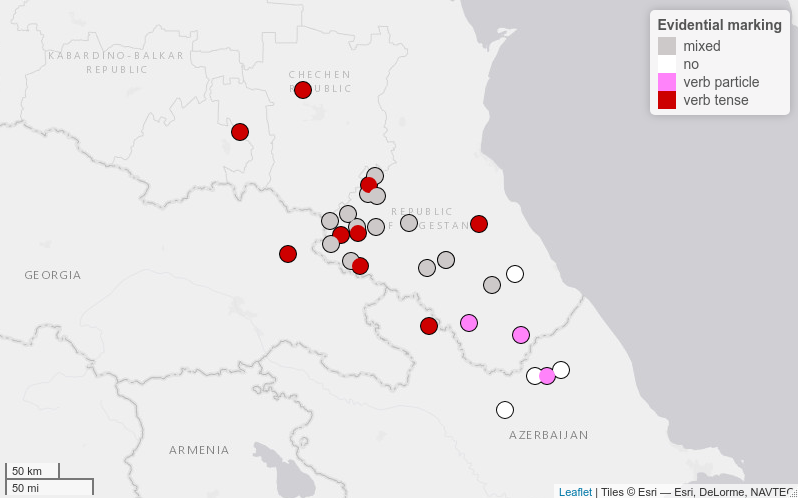
\includegraphics[scale=0.70]{images/system.png}}
\end{figure}

По нашим данным, смешанные системы более распространены: они находятся в 16/29 языков. В 7 языках эвиденциальность выражается только внутри видо-временной системы, а соотвествующие клитики не отмечены. В трех языках имеются только специализированные глагольные аффиксы. В трёх языках категория видимо отсутствует: в удинском, в будухском и в табасаранском. Из них удинский относительно хорошо изучен, так что можно с большой уверенностью предполагать, что категории эвиденциальности в нем нет. Ниже приводим более детальные карты, на которых разные способы (глагольные формы / частицы) изображены на отдельных картах.

На рисунке \ref{fig:evtensemap} показано, в каких языках эвиденциальность отмечается внутри видо-временной парадигмы (включая как несмешанные, так и смешанные системы). Цвет точки соответствует языку, а присутствие или отсутствие эвиденциальности указано цветом ободка.

\begin{figure}[H]
\centering
\caption{Эвиденциальность в видо-временной системе нахско-дагестанских языков}
\label{fig:evtensemap}
\vspace{0.5cm}
\fbox{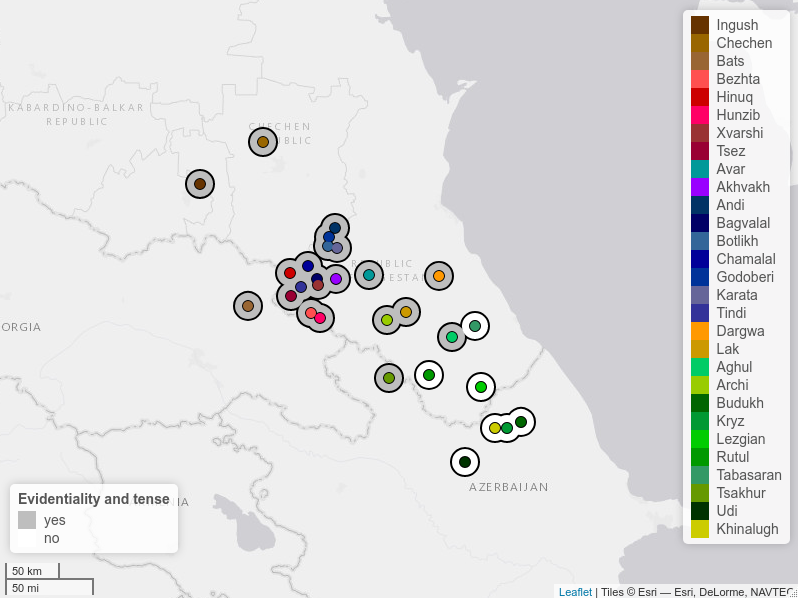
\includegraphics[scale=0.7]{images/tense.png}}
\end{figure}

На рисунке \ref{fig:evtensemap} можно заметить ареально-генеалогический паттерн. Среди лезгинских языков на юге региона признак отсутствует (исключениями являются цахурский и агульский языки). При этом мы знаем, что азербайджанский язык очень сильно влиял на языки этого региона. Эвиденциальность в видо-временной системе связана главным образом с перфектоидными формами, выражающими косвенную засвидетельствованность. Рисунок \ref{fig:evpfmap} показывает распределение перфектоидов с эвиденциальным значением и без него, показанное так же, как на предыдущей карте.

\begin{figure}[H]
\centering
\caption{Перфектоиды и эвиденциальность в нахско-дагестанских языках}
\label{fig:evpfmap}
\vspace{0.7cm}
\fbox{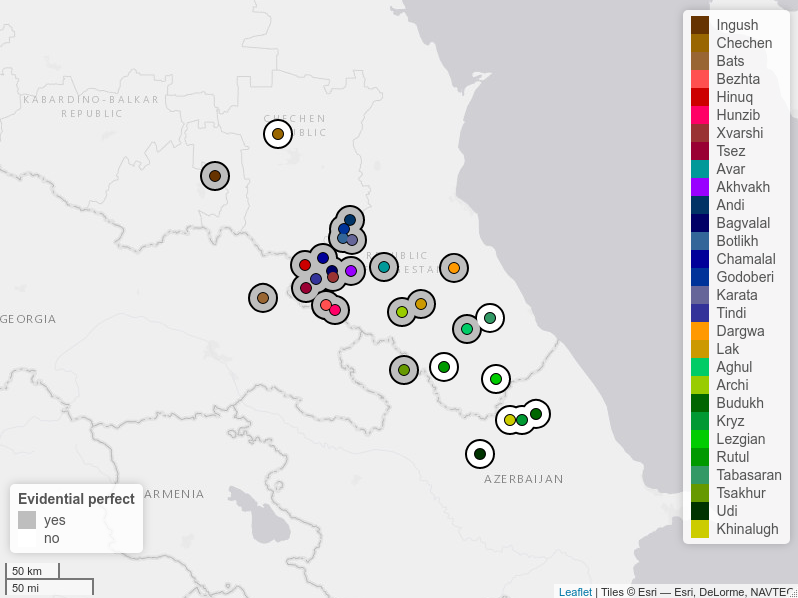
\includegraphics[scale=0.7]{images/perfectoids.png}}
\end{figure}

В данных о перфектоидах, которые представлены в разделе \ref{sec:perf}, было учтено несколько дополнительных диалектов; были проанализированы разные перфектоидные формы.\footnote{Точки, показанные на картах на рисунке \ref{fig:pfsemmap}, имеют разную природу. На предыдущих картах использовались координаты языков из базы данных Glottolog 4.0 \citep{glottolog}. Координаты Глоттолога представляют приближение примерного региона проживания носителей какого-то языка. Реальность, конечно, сложнее (ср. например рисунок \ref{fig:ecvill} в настоящей работе. В рисунке \ref{fig:pfsemmap} пункты из Глоттолога дополнены более точными сведениями там, где это возможно. Одноаульный ширинский даргинский, например, имеет координаты самого села Шари (по данным карт поисковой машины Гугл). В исходных данных указано, какого рода точка используется --- координаты определенного села или обобщенная точка по Глоттологу.} Карта показывают распределение перфектоидов на карте по семантическим признакам. Она отражает ареальные паттерны, аналогичные тем, которые наблюдаются выше на рис. \ref{fig:evtensemap}, \ref{fig:evpfmap}: на юге эвиденциальное значение у перфектоидов отсутствует (рис. \ref{fig:pfsemmap}), а результативное значение и текущая релевантность по контрасту представлены по всему региону.

\begin{figure}[H]
\centering
\caption{Значения перфектоидов в нахско-дагестанских языках}
\label{fig:pfsemmap}
\vspace{0.7cm}
\fbox{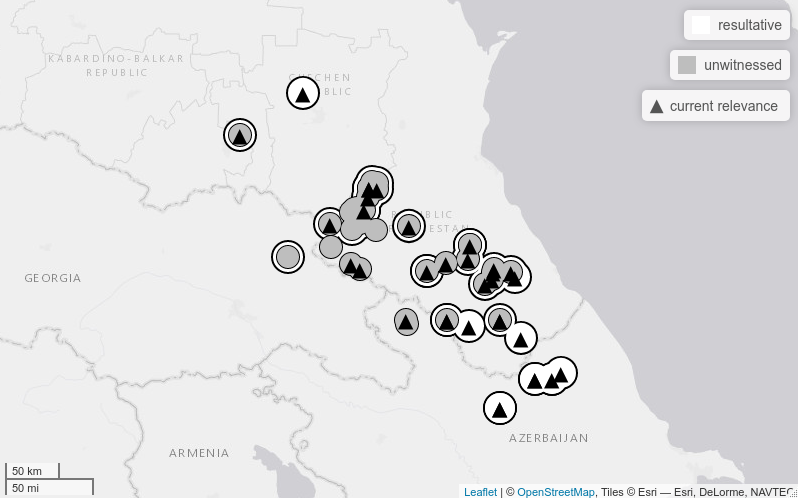
\includegraphics[scale=0.7]{images/pmeaning.png}}
\end{figure}

По сравнению с эвиденциальностью как значение перфектоида, эвиденциальные клитики, описанные в разделе \ref{sec:clitics} не показывают ярко ареальное распределение, ср. рисунки \ref{fig:tensepart} и \ref{fig:clitictype}.

\vfill
\pagebreak

\begin{figure}[H]
\centering
\caption{Эвиденциальность в видо-временной системе и клитики}
\label{fig:tensepart}
\vspace{0.7cm}
\fbox{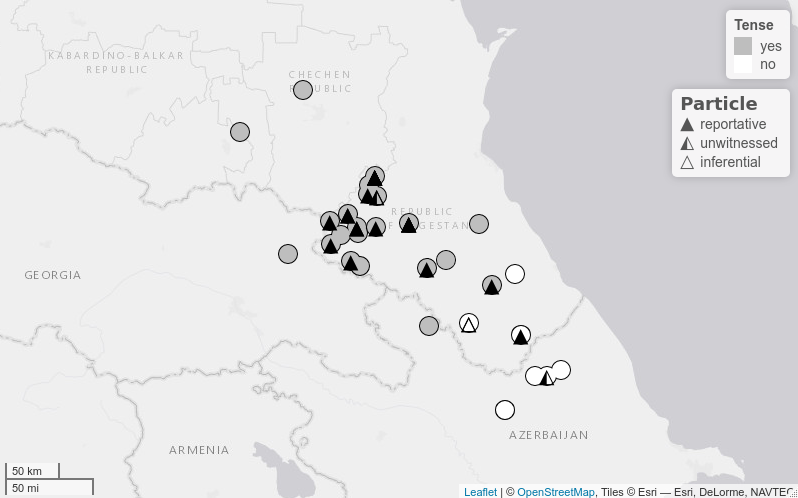
\includegraphics[scale=0.7]{images/tensep.png}}
\end{figure}

\begin{figure}[H]
\centering
\caption{Распространение эвиденциальных клитик}
\label{fig:clitictype}
\vspace{0.7cm}
\fbox{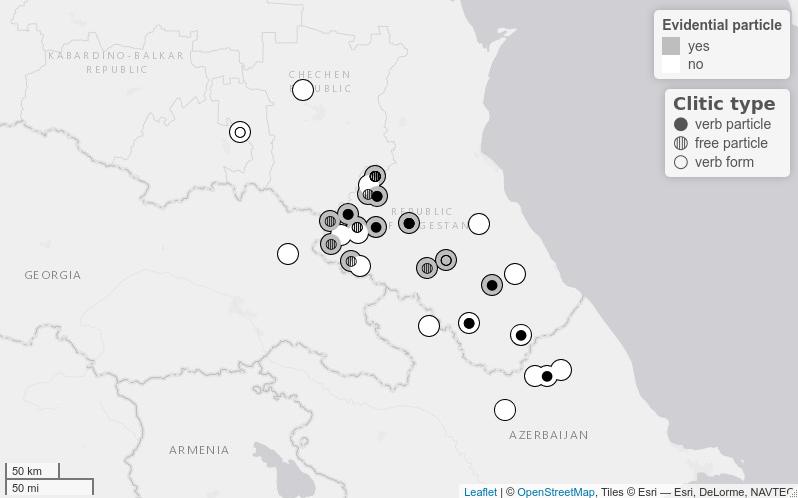
\includegraphics[scale=0.7]{images/ctype.png}}
\end{figure}


\subsection{Итоги} \label{sec:itogi2}

Эвиденциальность в нахско-дагестанских языках появляется в первую очередь как одно из значений перфектоидных форм. Эти формы обладают разной степенью конвенционализации и грамматикализации эвиденциального значения. Все они происходят из результативной конструкции, чаще всего на основе (общего перфективного) конверба и копулы. В некоторых, но не во всех языках при этом используются когнатные единицы. Представлены и другие варианты оформления функционально аналогичной конструкций, в том числе конструкции на основе причастия или суффиксальной конструкции неизвестного происхождения. В целом складывается впечатление, что перфектоидные формы в нахско-дагестанских языках не сводятся к единому источнику в праязыке, но представляют собой параллельный дрейф, причем пути их эволюции и организация парадигмы в разных языках могут достаточно сильно различаться: с одной стороны, одна форма может сочетать все возможные значения перфектоида (результатив, текущая релевантность, косвенная засвидетельствованность), с другой стороны, в языке может быть одновременно представлено несколько более специализированных форм. Специализированные узкие результативы в нахско-дагестанских языках отличаются от форм текущей релевантности тем, что они не допускают присутствие действующего субъекта, см. раздел \ref{sec:res}. Эвиденциальная функция и функция текущей релевантности, в типологических подходах часто считающаяся прототипической функцией перфекта, в нахско-дагестанских языках обе хорошо представлены. При этом, если семантика ТР распространена по всему региону, эвиденциальность как значение перфектоида на юге Дагестана в основном отсутствует. Тот факт, что данное значение здесь не отмечается, по-видимому, не является результатом неполноты описаний, что подтверждается подробным исследованием \citep{maisaklezgpf}.
\par Любопытное ареальное распределение признака косвенной засвидетельствованности как значения перфектоида, по контрасту с распределением разного рода эвиденциальных клитик, как обсуждалось в разделе (\ref{sec:maps}). Тем не менее, сравнение описаний форм в нахско-дагестанских языках с соответсвующими формами из тюркских языков не позволяет предполагать, что данный признак, в тех языках, где он присутствует, появился под влиянием контакта с тюркскими языками, по разным причинам. Во-первых, в дагестанских тюркских языках косвенная засвидетельствованность, по всей видимости, слабо выражена. Во-вторых, если какое-то заимствование из тюркских языков имело место, то речь идет о заимствовании дополнительного компонента значения у частично аналогичной формы (см. раздел \ref{sec:dagturk}), что представляет собой достаточно сложный процесс. Нахско-дагестанские перфектоиды формально сильно отличаются от тюркских: в тюркских языках выражение косвенной засвидетельствованности осуществляется конструкциями на основе причастий, тогда как для нахско-дагестанских языков более характерны конвербы. При этом в нахско-дагестанских языках широко представлены аналитические формы, в то время как аналитическое происхождение тюркских конструкций не доказано. В-третьих, несмотря на то, что признак скорее всего не сводится к уровню праязыка или даже праязыков разных групп, и он подозрительно частотен на Кавказе, нельзя опровергать сценарий, что он развивался самостоятельно в отдельных языках, особенно при отсутствии исторических данных о языках и языковых контактах. Тем не менее, можно обнаружить два ареала в данном регионе, которые включают в себя тюркские языки: северо-западная / центральная зона, где признак наличествует, и южная зона, где он отсутствует. 
\par В разделе \ref{sec:ndlang} было отмечено, что влияние мусульманской культуры и исламизации шло с юга на север, что отражается и в местном фольклоре: на севере до какой-то степени сохранены фольклорные мотивы, которые характерны для разных народов Северного Кавказа и которые предшествовали исламизацию, тогда как на юге они не представлены. Напомним, что тюркские народы играли важную роль в распространение ислама и исламской культуры на этой территории. В частности, азербайджанский язык служил важным посредником между нахско-дагестанскими и иранским языками. Вместе с исламизацией пришли письменность и новые литературные формы. Возможно, определенную роль в распространении эвиденциального употребления перфектоидов (или его отсутствия) играла именно литература. В конвенционализованных нарративных жанрах эвиденциальные показатели используются особенно часто, а функция их в таких контекстах наиболее ярко выражена. В третьей главе мы рассмотрим употребление перфектоидов в фольклоре и в нарративных текстах. Там же обсуждается сценарий, при котором присутствие тех или иных тюркских языков могло способствовать или препятствовать развитию заглазной семантики.


